\documentclass[a4paper]{article}

\usepackage[14pt]{extsizes}
\usepackage[T2A]{fontenc}
\usepackage[russian]{babel}

\usepackage[left=20mm, top=15mm, right=15mm, bottom=20mm]{geometry}
\usepackage{listings}
\usepackage{tikz}
\usetikzlibrary{shapes.geometric, arrows.meta, positioning, calc, arrows, shapes.misc}
\usepackage{graphicx}
\usepackage{amsmath, amssymb} % For equations
\usepackage{booktabs} % For better tables
\usepackage{pgfplots} % For plotting graphs
\usepackage{caption} % For captioning tables and figures
\usepackage{float} % For precise float placement (images, tables)
\usepackage[hidelinks]{hyperref} % For table of contents to be clickable
\usepackage{bookmark}
\usepackage{multirow}
\usepackage{array}
\usepackage{cancel}
\usepackage{placeins}
\usepackage{enumitem}
\usepackage{makecell}
\pgfplotsset{compat=1.17}
\usepackage{circuitikz}
\usetikzlibrary{decorations.markings} % For custom arrow positioning
\definecolor{good}{HTML}{C6EFCE}    % bright green
\definecolor{neutral}{HTML}{FFFFCC} % bright yellow
\definecolor{bad}{HTML}{FFC7CE}     % bright red
\usepackage[table]{xcolor}
\usepackage{wrapfig}
\usepackage{titlesec}
% \titleformat{\section}[hang]{\large\bfseries}{\thesection.}{1em}{}
% \titlespacing*{\section}{0pt}{*2}{*1}

% important macro for rounded corners in pictures
\newcommand{\cutpic}[3]{
	\savebox{\picbox}{\includegraphics[width=#2]{#3}}
	\tikz\node [draw, rounded corners=#1, line width=4pt,
		color=white, minimum width=\wd\picbox,
		minimum height=\ht\picbox, path picture={
				\node at (path picture bounding box.center) {
					\usebox{\picbox}};
			}] {};}

% -----------------------------------------------------

\newcommand{\labtitle}[9]{
	\begin{center}
		\vspace*{-1.8cm}
		
\includegraphics[width=0.26\textwidth]{../common/itmo-logo.png}\\
		\vspace{2.4cm}
		\textbf{\Large Основы электротехники}\\[1.2cm]
		\textbf{\Large Отчёт по лабораторной работе №#1}\\[0.7cm]
		\textbf{\Large #2}\\[3cm]

		\textbf{\Large Группа \textcolor{red}{\textit{P#3}}}\\[0.2cm]
		\textbf{\Large Вариант \textcolor{red}{\textit{#4}}}\\[3cm]

		\begin{flushleft}
			\textbf{\large Выполнил: \textcolor{red}{\textit{#5}}}\\[0.5cm]
			\textbf{\large Дата сдачи отчёта: \textcolor{red}{#6}}\\[0.5cm]
			\textbf{\large Дата защиты: \textcolor{red}{#7}}\\[0.5cm]
			\textbf{\large Контрольный срок защиты: \uline{#8}}\\[0.5cm]
			\textbf{\large Количество баллов: \uline{#9}}\\[2cm]
		\end{flushleft}
	\end{center}

	\vspace*{\fill}
	\begin{center}
		\textbf{\Large СПб -- 2024}
	\end{center}
	\vspace*{-1.8cm}
}

\newcommand{\hwtitle}[8]{
	\begin{center}
		\vspace*{-1.8cm}
		
\includegraphics[width=0.26\textwidth]{../common/itmo-logo.png}\\
		\vspace{2.4cm}
		\textbf{\Large Основы электротехники}\\[1.2cm]
		\textbf{\Large Домашнее задание №#1}\\[0.7cm]
		\textbf{\Large #2}\\[3cm]

		\textbf{\Large Группа \textcolor{red}{\textit{P#3}}}\\[0.2cm]
		\textbf{\Large Вариант \textcolor{red}{\textit{#4}}}\\[3cm]

		\begin{flushleft}
			\textbf{\large Выполнил: \textcolor{red}{\textit{#5}}}\\[0.5cm]
			\textbf{\large Дата сдачи: \textcolor{red}{#6}}\\[0.5cm]
			\textbf{\large Контрольный срок сдачи: \uline{#7}}\\[0.5cm]
			\textbf{\large Количество баллов: \uline{#8}}\\[2cm]
		\end{flushleft}
	\end{center}

	\vspace*{\fill}
	\begin{center}
		\textbf{\Large СПб -- 2024}
	\end{center}
	\vspace*{-1.8cm}
}

% % listing for programming code blocks
\lstset{
	language=C++,                 % Programming language
	basicstyle=\ttfamily\normalsize, % Adjust font size
	keywordstyle=\color{blue},    % Style for keywords
	stringstyle=\color{red},      % Style for strings
	commentstyle=\color{gray},   % Style for comments
	morecomment=[l][\color{magenta}]{\#}, % Special comment style
	breaklines=true,              % Line breaking in long lines
	numbers=left,                 % Line numbering on the left
	numberstyle=\tiny\color{gray},% Style for line numbers
	frame=single,                 % Code frame
	showstringspaces=false        % Don't show spaces in strings
}

% % tikz styles for flowcharts
\tikzset{
	startstop/.style={
			rectangle,
			rounded corners,
			minimum width=3cm,
			minimum height=1cm,
			text centered,
			draw=black,
			fill=red!30
		},
	io/.style={
			trapezium,
			trapezium left angle=70,
			trapezium right angle=110,
			minimum width=3cm,
			minimum height=1cm,
			text centered,
			draw=black,
			fill=blue!30
		},
	process/.style={
			rectangle,
			minimum width=3cm,
			minimum height=1cm,
			text centered,
			draw=black,
			fill=orange!30
		},
	decision/.style={
			diamond,
			aspect=2,
			minimum width=3cm,
			text centered,
			draw=black,
			fill=green!30
		},
	arrow/.style={
			thick,
			->,
			>=stealth
		},
	prep/.style={
			chamfered rectangle,
			chamfered rectangle xsep=2cm,
			draw,
			thick,
			minimum width=5cm,
			minimum height=1cm,
			text centered,
			text width=2.5cm,
			font=\small,
			fill=yellow!30
		},
}


\begin{document}

% Title page
% old basic group uir title
\begin{center}
	\vspace{1cm}
	\large{Университет ИТМО}\\
	\large{Факультет программной инженерии и компьютерной техники}\\
	\vspace{4cm}
	\Large{\textbf{Учебно-исследовательская работа №1 (УИР 1)\\}}
	\vspace{0.3cm}
	\large{\textbf{<<Кодирование данных в телекоммуникационных системах>>\\}}
	\vspace{-0.3cm}
	\begin{center}
		\large{по дисциплине <<Телекоммуникационные системы>>}
	\end{center}
	\vspace{3cm}
\end{center}
\normalsize{
	\begin{flushright}
		Выполнил:
		\par
		Студент 3 курса группы P3331
		\par
		Дворкин Борис Александрович
		\par
		\textbf{Вариант: ДвБА}
		\par
		\vspace{1cm}
		Преподаватель:
		\par
		Алиеф Тауфик Измайлович
		\par
		\noindent Отчёт принят «\underline{\hspace{0.7cm}}» \underline{\hspace{1.3cm}} 2024 г.\\
		Оценка: \underline{\hspace{2cm}}
	\end{flushright}
}\\
\vspace{6cm}
\begin{center} г. Санкт-Петербург
	\par
	2024 г.
\end{center}
\thispagestyle{empty}
\thispagestyle{empty}


% -------------------------------

\newpage
\pagestyle{plain}
\setcounter{page}{1} % Enable text numbering

% -------------------------------

% autogenerated table of contents
\linespread{0.9}
\tableofcontents
\linespread{1}

% -------------------------------

\newpage
\section*{Цель работы}
\addcontentsline{toc}{section}{Цель работы}
Исследование влияния свойств канала связи на качество передачи сигналов при различных методах \textit{физического} и \textit{логического} кодирования, используемых в цифровых сетях передачи данных.


% -------------------------------

\section{Формирование сообщения}
\begin{enumerate*}
\item ФИО: Дворкин Борис Александрович

\item Исходное сообщение: \textbf{ДвБА}

\item Сообщение состоит из 4 символов: Д, в, Б, А.

\begin{center}
	\begin{tabular}{|c|c|c|}
		\hline
		\textbf{Символ} & \textbf{В шестнадцатеричном коде} & \textbf{В двоичном коде} \\
		\hline
		Д               & C4                                & 1100\ 0100               \\
		в               & E2                                & 1110\ 0010               \\
		Б               & C1                                & 1100\ 0001               \\
		А               & C0                                & 1100\ 0000               \\
		\hline
	\end{tabular}
\end{center}

\item Итоговое сообщение в шестнадцатеричном коде:
\[
	\textbf{C4 E2 C1 C0}
\]

\item Итоговое сообщение в двоичном коде:
\[
	\textbf{1100 0100 1110 0010 1100 0001 1100 0000}
\]

\item Длина итогового сообщения: \textbf{4 байт (32 бит)}
\end{enumerate}


% -------------------------------

\section{Минимальная полоса пропускания канала \-связи}
Во избежание повторений продемонстрирую как выглядит моё сообщение, закодированное с помощью потенциального метода NRZ:
Для определения верхней границы частот необходимо найти наиболее высокочастотную составляющую спектра в передаваемом сообщении, которая в NRZ образуется при передаче чередующихся значений 0 и 1, при этом период гармонического сигнала (синусоиды), используемого для передачи прямоугольных сигналов 0 и 1, будет равен удвоенной длительности битового интервала $\tau: T = 2\tau$, где $\tau$ определяется как величина, образная значению пропускной способности канала $C: \tau = \frac{1}{C}$. Отсюда верхняя граница частот будет равна \[f_{\text{в}} = \frac{1}{T} = \frac{C}{2}\]

То есть, при пропускной способности канала связи $C = 10 \, \text{Мбит/с}$ частота основной гармоники равна $f_{\text{в}} = \frac{10 \cdot 10^3}{2} = 5 \, \text{МГц}$, а битовый интервал $\tau = 100 \, \text{нс}$.

В общем случае, при кодировании любого сообщения с помощью метода NRZ наибольшая (верхняя) частота достигается при передаче чередующихся значений 0 и 1, а наименьшая (нижняя) - при передаче длинных (в пределе - бесконечных) последовательностей нулей и единиц, что делает нижнюю границу частот близкой и в пределе равной нулю: $f_{\text{н}} = 0$. Следовательно, в предельном случае спектр: $S = f_{\text{в}} - f_{\text{н}} = f_{\text{в}} = \frac{C}{2}$.

С другой стороны, при передаче конкретного сообщения нижняя частота всегда больше нуля и зависит от максимальной длины последовательностей нулей или единиц. В этом случае для расчёта нижней границы чапстот необходимо в коде передаваемого сообщения найти \textit{наиболее длинную последовательность 1 или 0}. В исходном сообщении, закодированном по методу NRZ, представленному на рисунке 1, низкочастотная составляющая образуется при передаче 6 последовательных нулей. Период синусоидального сигнала при передаче таких последовательностей равен 12 битовым интервалам и нижняя граница частот соответственно будет равна: $f_{\text{н}} = \frac{1}{12\tau} = \frac{C}{12}$. Тогда \textbf{спектр} при передаче данного сообщения кодом NRZ равен
\[
	S =  f_{\text{в}} - f_{\text{н}} = \frac{C}{2} - \frac{C}{12} = \frac{5C}{12} = 4.167 \, \text{МГц}
\]

Среднее значение частоты передаваемого сообщения находится в интервале $(f_{\text{н}};f_{\text{в}})$ и показывает, какие частоты (низкие или высокие) превалируют в спектре передаваемого сигнала.

Для оценки среднего значения частоты передаваемого сообщения можно для каждого битового интервала определить соответствующую частоту сигнала, просуммировать их и разделить на количество битовых интервалов. В нашем случае: частота основной гармоники $f_0 = \frac{C}{2}$ соответствует трём битовым интервалам, частота вдвое меньшая, т.е. $\frac{f_0}{2}$, соответствует также трём битовым интервалам, частота $\frac{f_0}{3}$ - четырём битовым интервалам, $\frac{f_0}{5}$ - одному битовому интервалу, и $\frac{f_0}{6}$ - одному битовому интервалу.

Тогда средняя частота рассматриваемого сообщения
\[
	f_{\text{ср}} = \left(3f_0+3\frac{f_0}{2}+4\frac{f_0}{3}+\frac{f_0}{5}+\frac{f_0}{6}\right)/ 12 = \frac{31f_0}{60} = \frac{31 \cdot 5}{60} \approx 2.583 \, \text{МГц}
\]

Поскольку середине спектра рассматриваемого сообщения соответствует частота
\[
	f_{1/2} = (f_{\text{н}} + f_{\text{в}}) /2 = \frac{\frac{C}{2} + \frac{C}{12}}{2} = \frac{7C}{24} = 2.917 \, \text{МГц}
\]
Можно констатировать, что в спектре сигнала \textit{незначительно превалируют низкие частоты}: $f_{\text{ср}} < f_{1/2}$.

Для качественной передачи двоичных сигналов по реальному каналу связи и возможности их распознавания на приёмной стороне с минимальным количеством ошибок, желательно на передающей стороне формировать сигналы, приближающиеся к прямоугольной форме. Однако, спектр таких сигналов оказывается слишком большим. Можно показать, что для качественного распознавания сигнала на приемной стороне при передаче чередующихся значений 0 и 1 достаточно сформировать сигнал, содержащий первые 4 гармоники (поскольку более высокочастотные гармоники оказывают незначительное влияние на результирующий сигнал) с частотами $f_0=\frac{C}{2}, f_1=3f_0, f_2=5f_0, f_3=7f_0$. В этом случае верхняя граница частот $f_{\text{в}}=7f_0$, а ширина спектра сигнала при передаче рассматриваемого сообщения соответственно будет равна $S = f_{\text{в}} - f_{\text{н}} = 7f_0-f_0/6=41f_0/6=34.167 \, \text{МГц}$.

Итак, при пропускной способности канала связи $C = 10 \, \text{Мбит/с}$ верхняя и нижняя границы частот в передаваемом сообщении равны соответственно $f_{\text{в}} = 5 \, \text{МГц}$ и $f_{\text{н}} = 0.833 \, \text{МГц}$, спектр сигнала $S = 4.167 \, \text{МГц}$, среднее значение частоты в спектре передаваемого сигнала $f_{\text{ср}} = 2.583 \, \text{МГц}$, полоса пропускания, необходимая для качественной передачи данного сообщения $F=35 \, \text{МГц}$.


Так должен выглядеть полученный сигнал при отсутствии ошибок.

\subsection{NRZ}

Для потенциального метода кодирования NRZ определим минимальную требуемую полосу пропускания \textit{идеального канала связи} для качественной передачи сообщения:
\begin{enumerate}
	\item Отсутствуют шумы и помехи
	\item Принимающие и передающие узлы абсолютно синхронизированны
	\item Сигналы не затухают $\Rightarrow$ не нужно устанавливать уровни граничного напряжения
\end{enumerate}

Следовательно, установим нулевые значения для Noise, Desync и Voltage в программе <<Network Fourier 23>>. Затем, введём исходное сообщение в шестнадцатеричном виде в обратном порядке, т.к. в таком порядке мы передаём сообщение по каналу связи. Далее, начнём передавать сообщение и подберём значения нижней и верхней гармоник спектра сигнала так, чтобы соответствующие им значения частот определяли границы минимальной полосы пропускания сигнала, то есть граничные значения, при которых ещё нету ошибок в процессе передачи.


\begin{wrapfigure}{l}{0.65\textwidth}
	\centering
	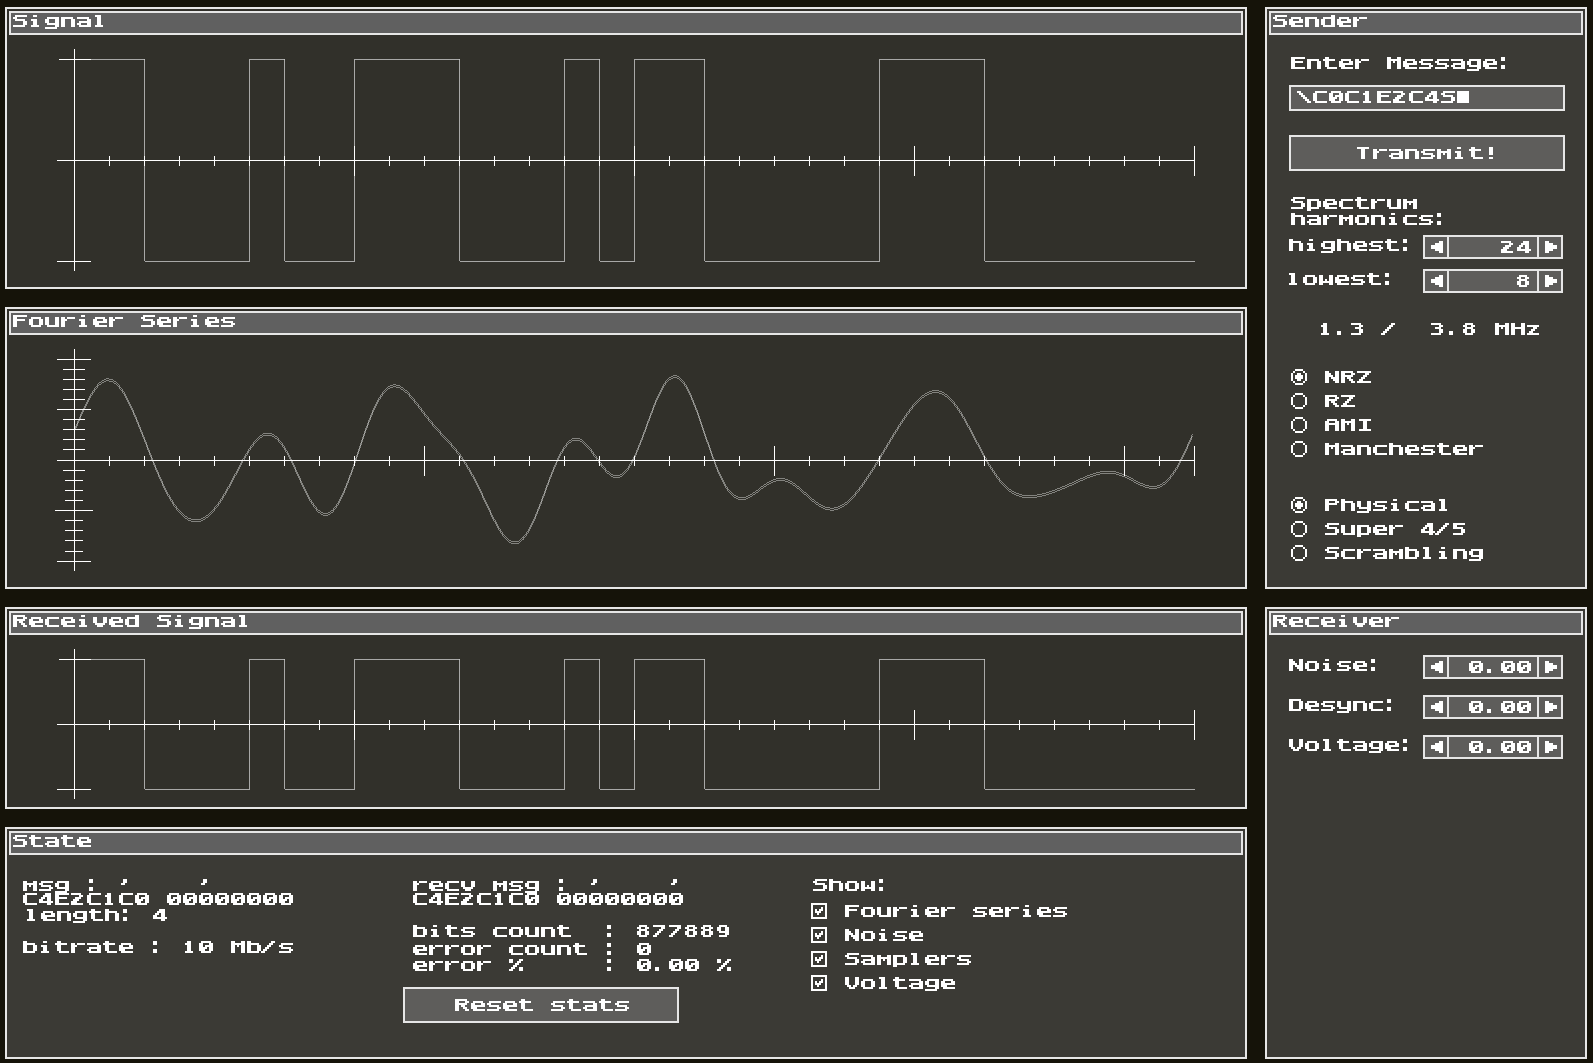
\includegraphics[width=0.95\linewidth]{./data/ideal_nrz_min_f.png}
	\caption{F = 1.3 - 3.8 Мгц}
\end{wrapfigure}

Для потенциальных методов кодирования, таких как NRZ или RZ, превалируют низкие частоты. При передаче конкретного сообщения нижняя частота всегда больше нуля и зависит от максимальной длины последовательностей нулей или единиц. В исходном сообщении, закодированном по методу NRZ, представленному на рисунке 1, низкочастотная составляющая образуется при передаче 6 последовательных нулей. Получается, что нижняя частота равна $\frac{C}{12}$, то есть при пропускной спобности $C = 10 \, \text{Мбит} / \text{с}$, указанной в программе, нижняя частота будет $\approx$ 0.83 Мгц. При этом верхняя граница частот будет образовываться при чередовании 0 и 1, что определяется из периода как $\frac{C}{2} = 5$ Мгц.

Проведя исследования, получили минимальную полосу пропускания идеального канала связи $F = 1.3 - 3.8 \, \text{Мгц}$. Спектр получился уже теоретического, в виду того, что это граничные значения, при которых вот-вот уже могут появиться ошибки. Для качественной предачи я бы значительно увеличил границу верхних частот, и уменьшил нижние частоты до рассчётных 0.8 Мгц.

\subsection{RZ}

\begin{wrapfigure}{r}{0.6\textwidth}
	\centering
	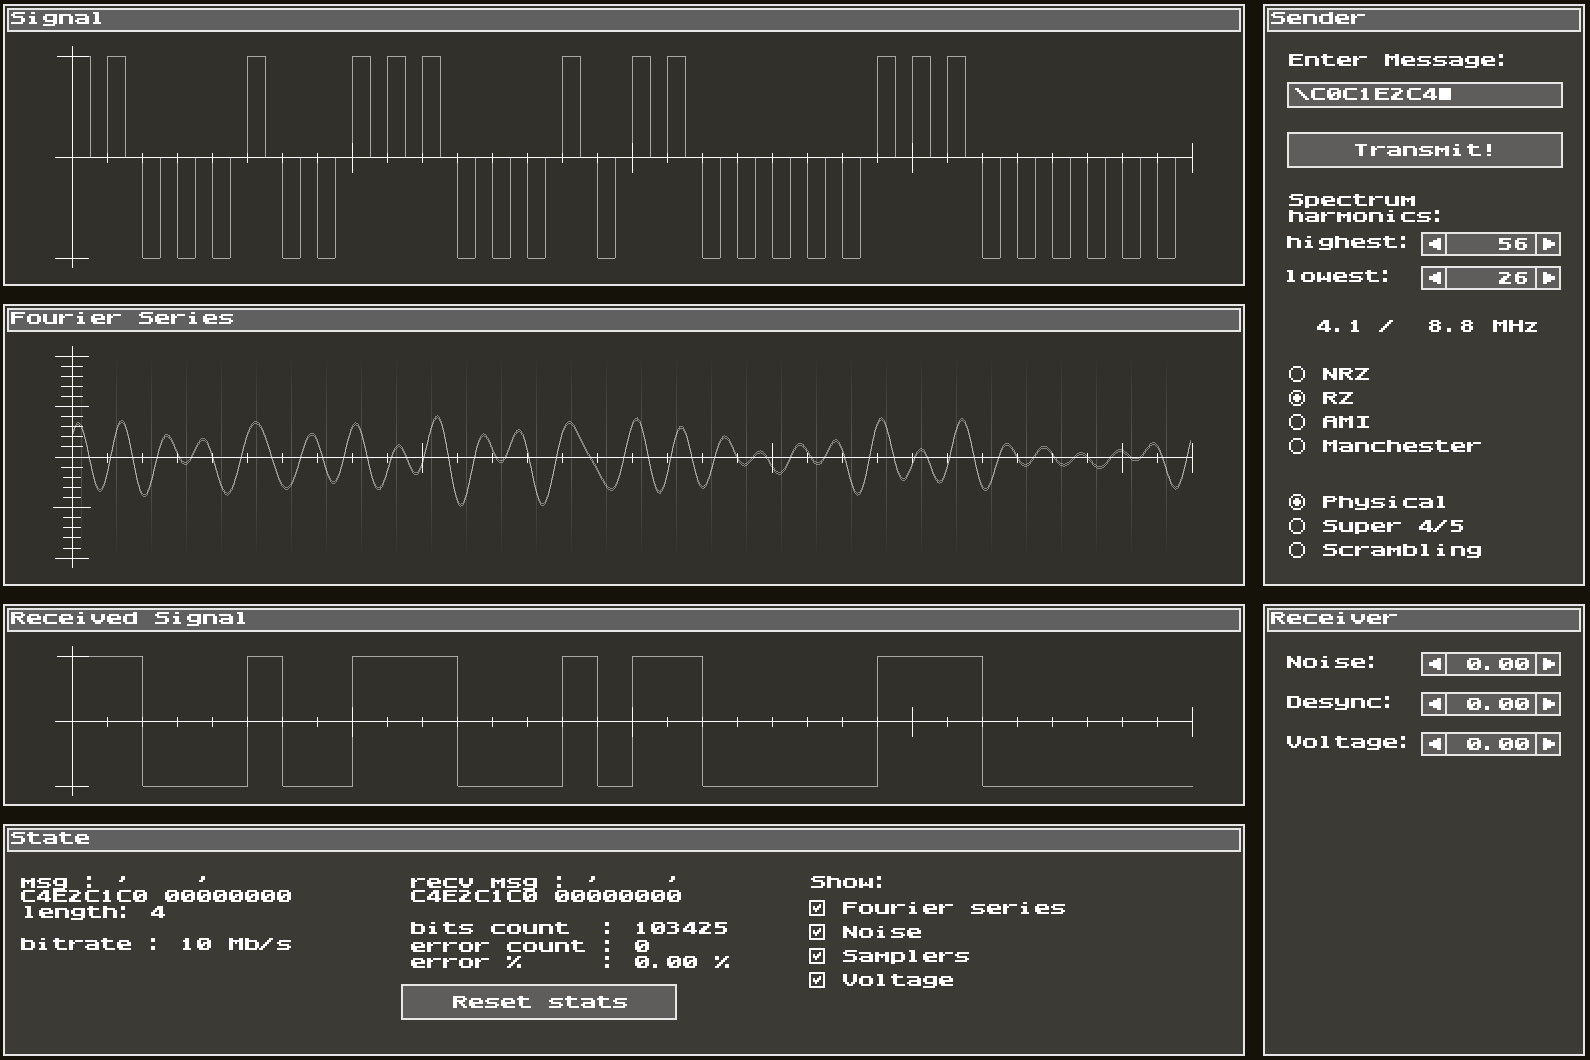
\includegraphics[width=0.95\linewidth]{./data/ideal_rz_min_f.png}
	\caption{F = 4.1 - 8.8 Мгц}
\end{wrapfigure}

Это тоже потенциальный метод кодирования, как и NRZ, поэтому низкочастотные особенности будут также иметь место и тут. В RZ верхняя частота достигается при передаче \textit{последовательных} значений 0 и 1, а нижняя - при передаче \textit{чередующихся} 0 и 1. период гармонического сигнала (синусоиды), используемого для передачи прямоугольных сигналов 0 и 1, будет равен длительности битового интервала $\tau$, умноженного на 5/2: $T = 2.5 \tau$. Тогда, нижняя граница частот $f_{\text{н}} = \frac{1}{T} = \frac{2C}{5}$, а верхняя $f_{\text{в}} = C$.


То есть, при пропускной способности канала связи $C = 10 \, \text{Мбит/с}$ частота основной гармоники равна $f_{\text{в}} = 10 \cdot 10^3 = 10 \, \text{МГц}$, битовый интервал $\tau = 100 \, \text{нс}$, $f_{\text{н}} = 4 \, \text{МГц}$. Следовательно, спектр: $S = f_{\text{в}} - f_{\text{н}} = 6 \, \text{МГц}$.

Проведя исследования, получили минимальную полосу пропускания идеального канала связи $F = 4.1 - 8.8 \, \text{Мгц}$, что уже теоретической в виду граничных, почти ошибочных значений. Для качественной предачи следует также значительно увеличить границу верхних частот, а нижние частоты практически совпали с рассчётными, что указывает на точность экспиримента.

\subsection{M2}

\begin{wrapfigure}{l}{0.58\textwidth}
	\centering
	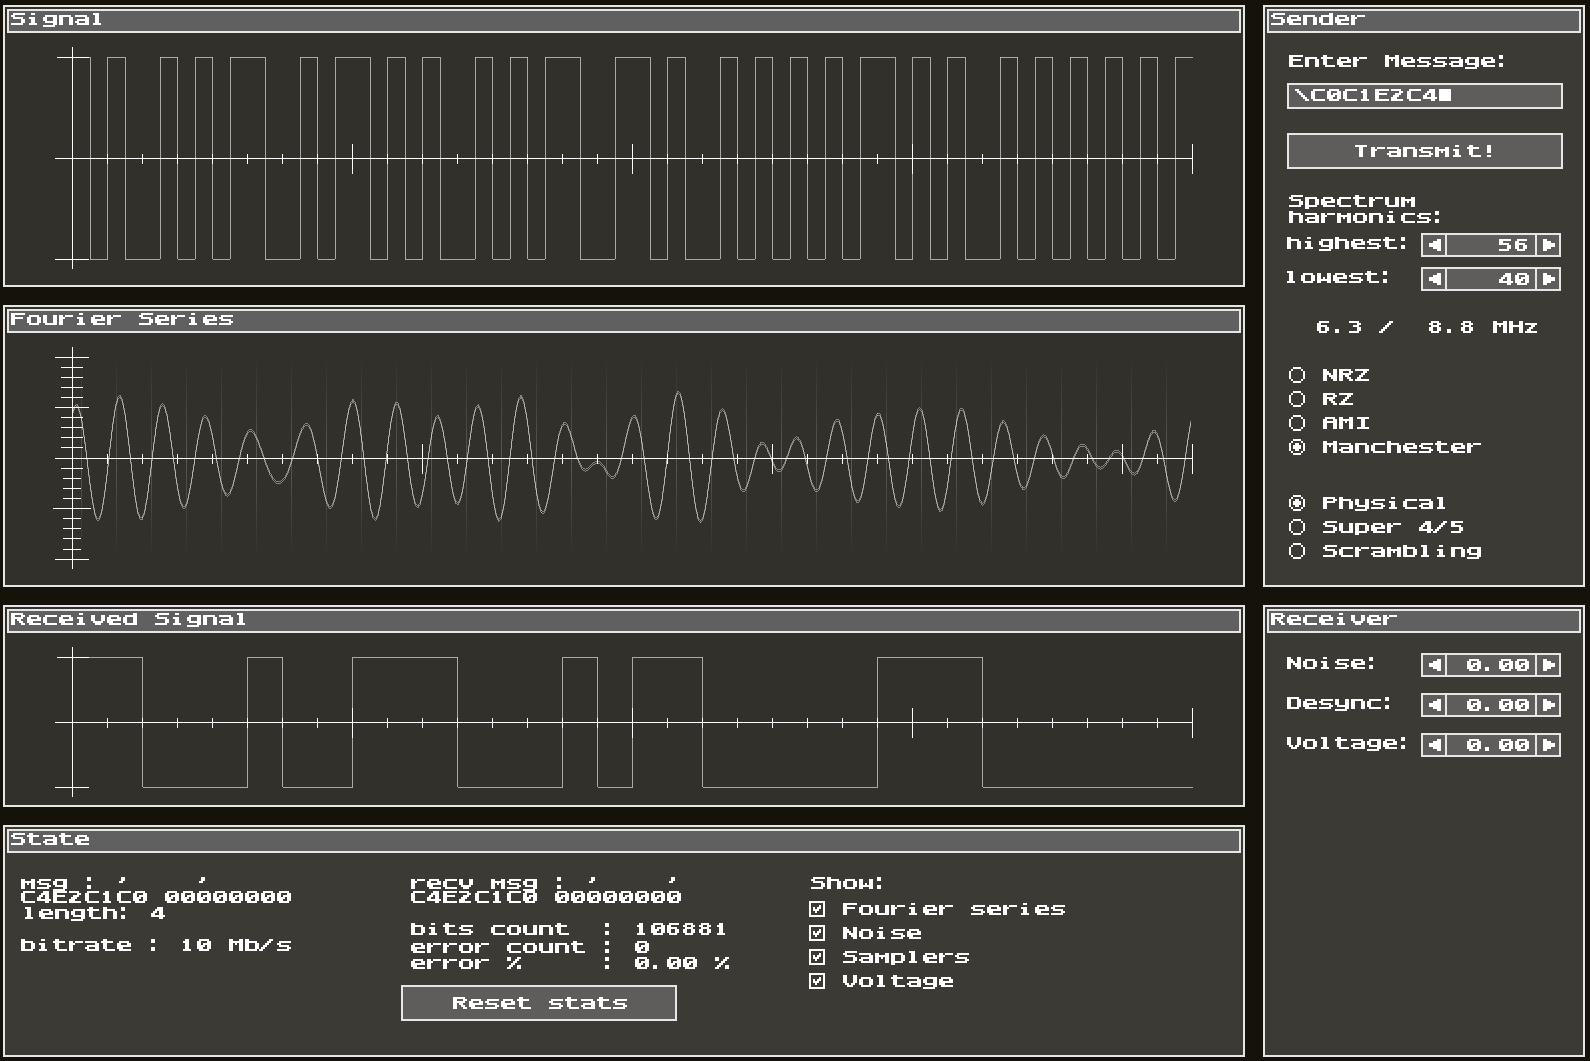
\includegraphics[width=0.95\linewidth]{./data/ideal_m2_min_f.png}
	% \cutpic{0.2cm}{9cm}{./data/ideal_m2_min_f.png}
	\caption{F = 6.3 - 8.8 Мгц}
\end{wrapfigure}

\vspace{-0mm}
Манчестерское кодирование - это импульсный метод кодирования. Это важное отличие от предыдущих методов, ведь кодирование сигнала импульсами позволяет избавиться от низкочастотных составляющих и соответственно их помех, а также улучшить синхронизацию.

Проведя аналогичные исследования, получили полосу в 2 раза уже теоретической, что демонстрирует повышенную устойчивость Манчестерского кодирования к помехам.

\subsection{Избыточное кодирование NRZ методом 4B/5B}

\newsavebox{\picbox}

Избыточное кодирование - это разновидность логического кодирования, применяемая в данном случае к потенциальному методу кодирования NRZ.

\begin{wrapfigure}{r}{0.6\textwidth}
	\centering
	\cutpic{0.2cm}{11cm}{./data/ideal_4b_5b.png}
	\caption{F =  2.0 - 4.5 Мгц}
\end{wrapfigure}


Суть избыточного кодирования - это улучшение синхронизации и устранение постоянной составляющей, которые присутствуют в моём сигнале при кодировании NRZ в виде последовательности повторяющихся значений <<0>> и/или <<1>>, с помощью замены каждых четырёх битов в исходном коде - пятью битами в результирующем, любое сочетание которых даёт 8 подряд расположенных <<1>> или 3 <<0>> в худшем случае.

Проведя исследования, получили минимальную полосу пропускания идеального канала связи $F = 2.0 - 4.5 \, \text{Мгц}$, что совпадает по ширине с минимальной полосой NRZ без избыточного кодирования, но отличается по диапазону частот - пришлось выполнять \textit{модуляцию} сигнала в более высокий диапазон частот.

\subsection{Скремблирование NRZ}

Сремблирование -  это также разновидность логического кодирования, суть которого заключается в применении определённого полинома к методу кодирования, в данном случае, NRZ, с целью уменьшения длинных последовательностей <<0>> и <<1>>.

\setlength{\intextsep}{0pt}
\setlength{\columnsep}{10pt}

\begin{wrapfigure}{r}{0.58\textwidth}
	\centering
	\cutpic{0.2cm}{11cm}{./data/ideal_nrz_scrambling.png}
	% 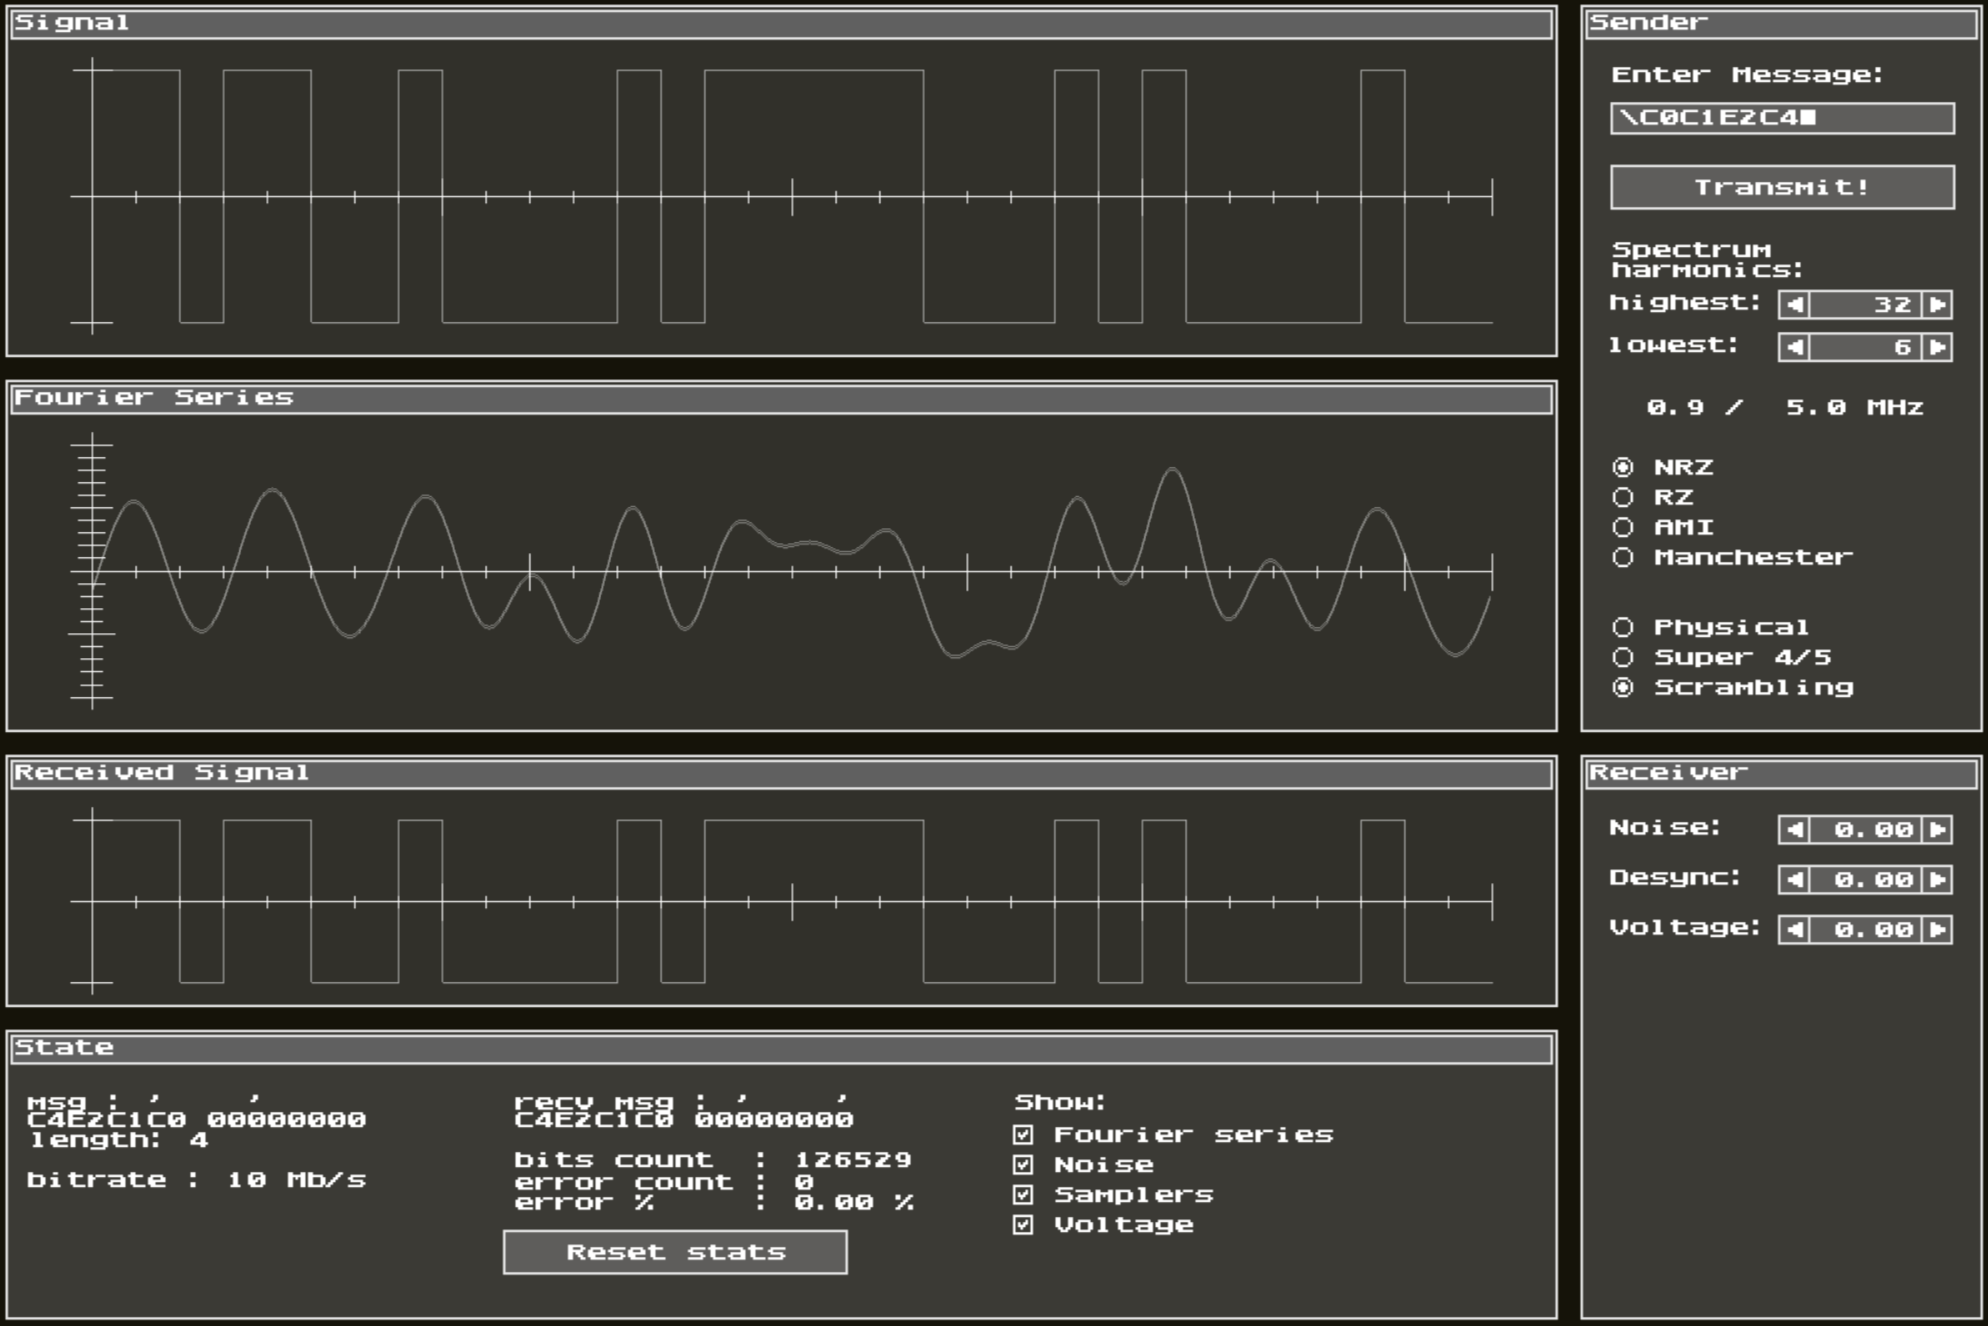
\includegraphics[width=0.95\linewidth]{./data/ideal_nrz_scrambling.png}
	\caption{F =  0.9 - 5.0 Мгц}
	\vspace{-140pt}
\end{wrapfigure}

Проведя исследования, получили минимальную полосу пропускания идеального канала связи $F = 0.9 - 5.0 \, \text{Мгц}$, то есть более широкую полосу пропускания, чем в базовом NRZ.

\newpage
\subsection{Выводы}

На этом этапе худший результат показал RZ – 4.7 МГц. Такая полоса пропускания связана с тем, что RZ имеет высокочастотную составляющую, а следовательно имеет большую полосу пропускания.

Метод NRZ оказался среди лучших – 2.5 МГц. При этом избыточное кодирование NRZ+4B/5B не изменило результат, а скремблирование ухудшило до 4.1 МГц. Таким образом, NRZ+4B/5B позволяет уменьшить влияние постоянной составляющей и добиться лучшей самосинхронизации и исправления ошибок, не сильно влияя на ширину полосы пропускания.

Несмотря на то, что в теории у M2 полоса пропускания шире остальных методов, для данного сообщения \underline{Манчестерское кодирование показало один из} \underline{лучших результатов – \textbf{2.5 МГц}}.


% -------------------------------

\newpage
\section{Допустимые уровни шума, рассинхронизации и затухания}
В ходе выполнения данного этапа я последовательно определял максимально допустимые уровни шумов, рассинхронизации и граничного напряжения, при которых сохраняется качественная передача сообщения.

Сначала я изменял уровень шумов \textbf{Noise} и определял его максимально допустимое значение при нулевых значениях остальных параметров.

Затем устанавливал уровень шумов в ноль и изменял уровень рассинхронизации \textbf{Desync}. Находил его максимально допустимое значение, при котором сообщение передается без ошибок.

Затем при нулевых значениях шумов и рассинхронизации я изменял уровень граничного напряжения \textbf{Voltage} и определял его максимально допустимое значение.


\subsection{NRZ}

\subsubsection{Noise}

Максимально допустимый уровень шума был определён с помощью программы \textit{Network Fourier} и составил \textbf{0.2}. Это граничное значение, при котором сигнал не искажается при воздействии произвольных гармоник.

\vspace{0.4cm}
\begin{figure}[h]
	\centering
	% 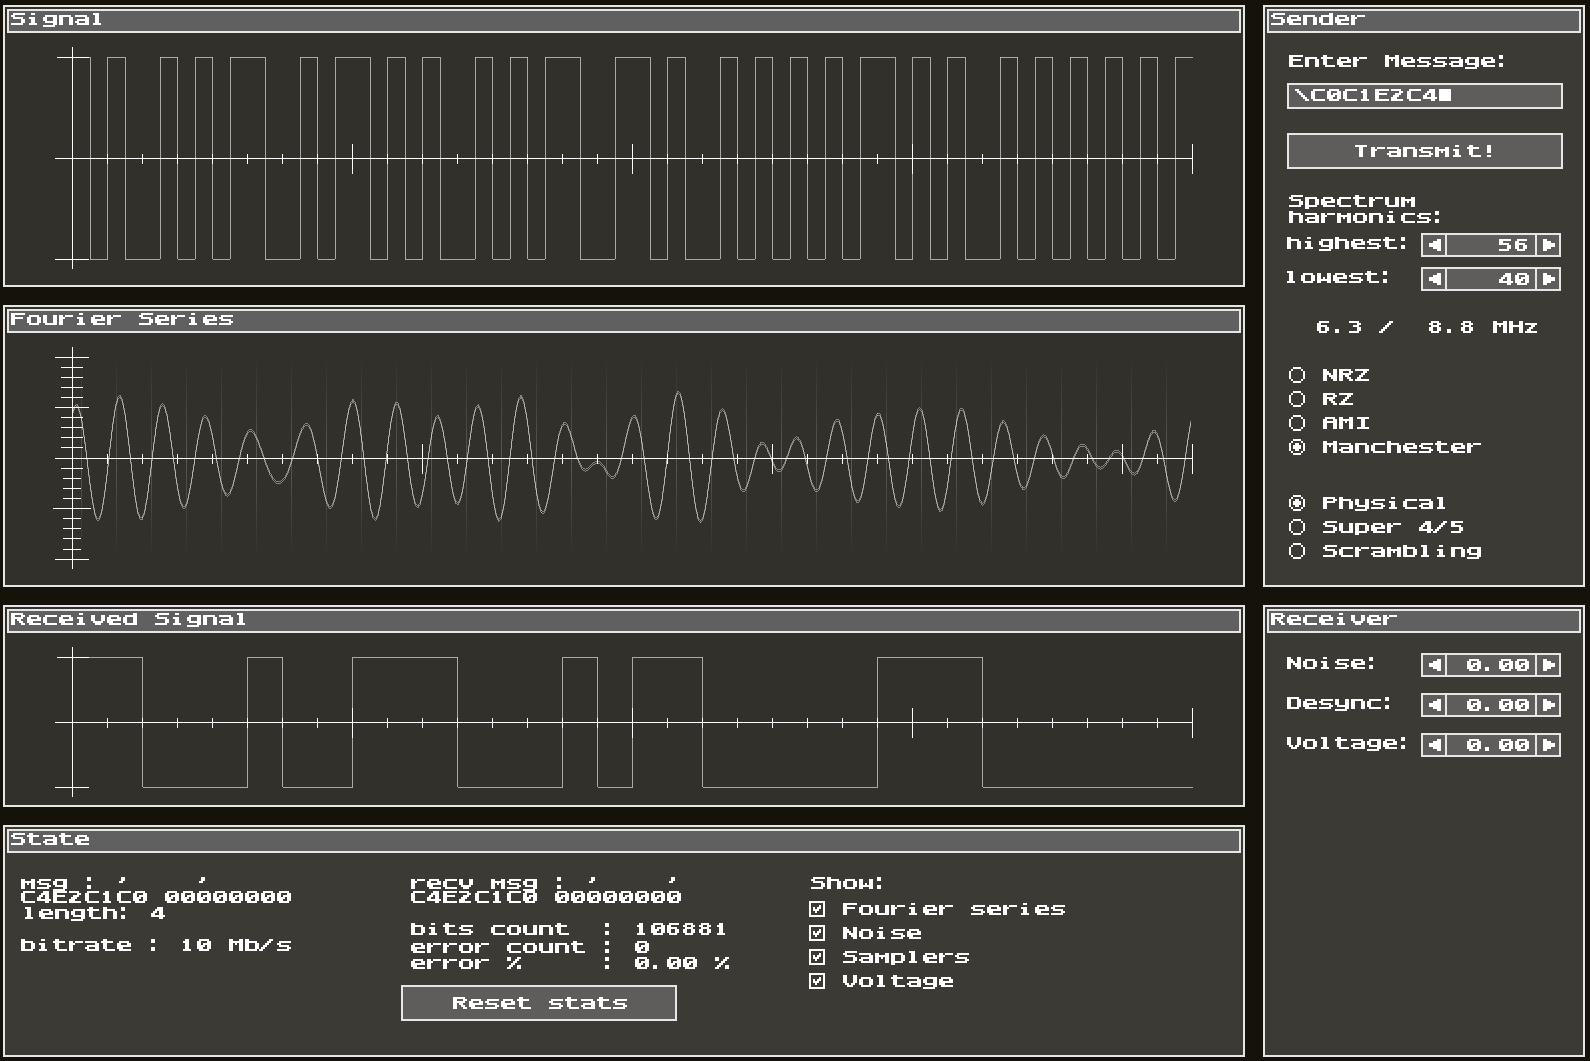
\includegraphics[width=0.95\linewidth]{./data/ideal_m2_min_f.png}
	\cutpic{0.2cm}{17cm}{./data/noise_nrz.png}
	\caption{Максимально допустимый уровень шума 0.2 для NRZ}
\end{figure}

\subsubsection{Desync}

Максимально допустимый уровень рассинхронизации был определён с помощью программы \textit{Network Fourier} и составил \textbf{0.35}. Это граничное значение, при котором различие часов передатчика и приёмника не искажают сигнал.

\vspace{0.4cm}
\begin{figure}[h]
	\centering
	% 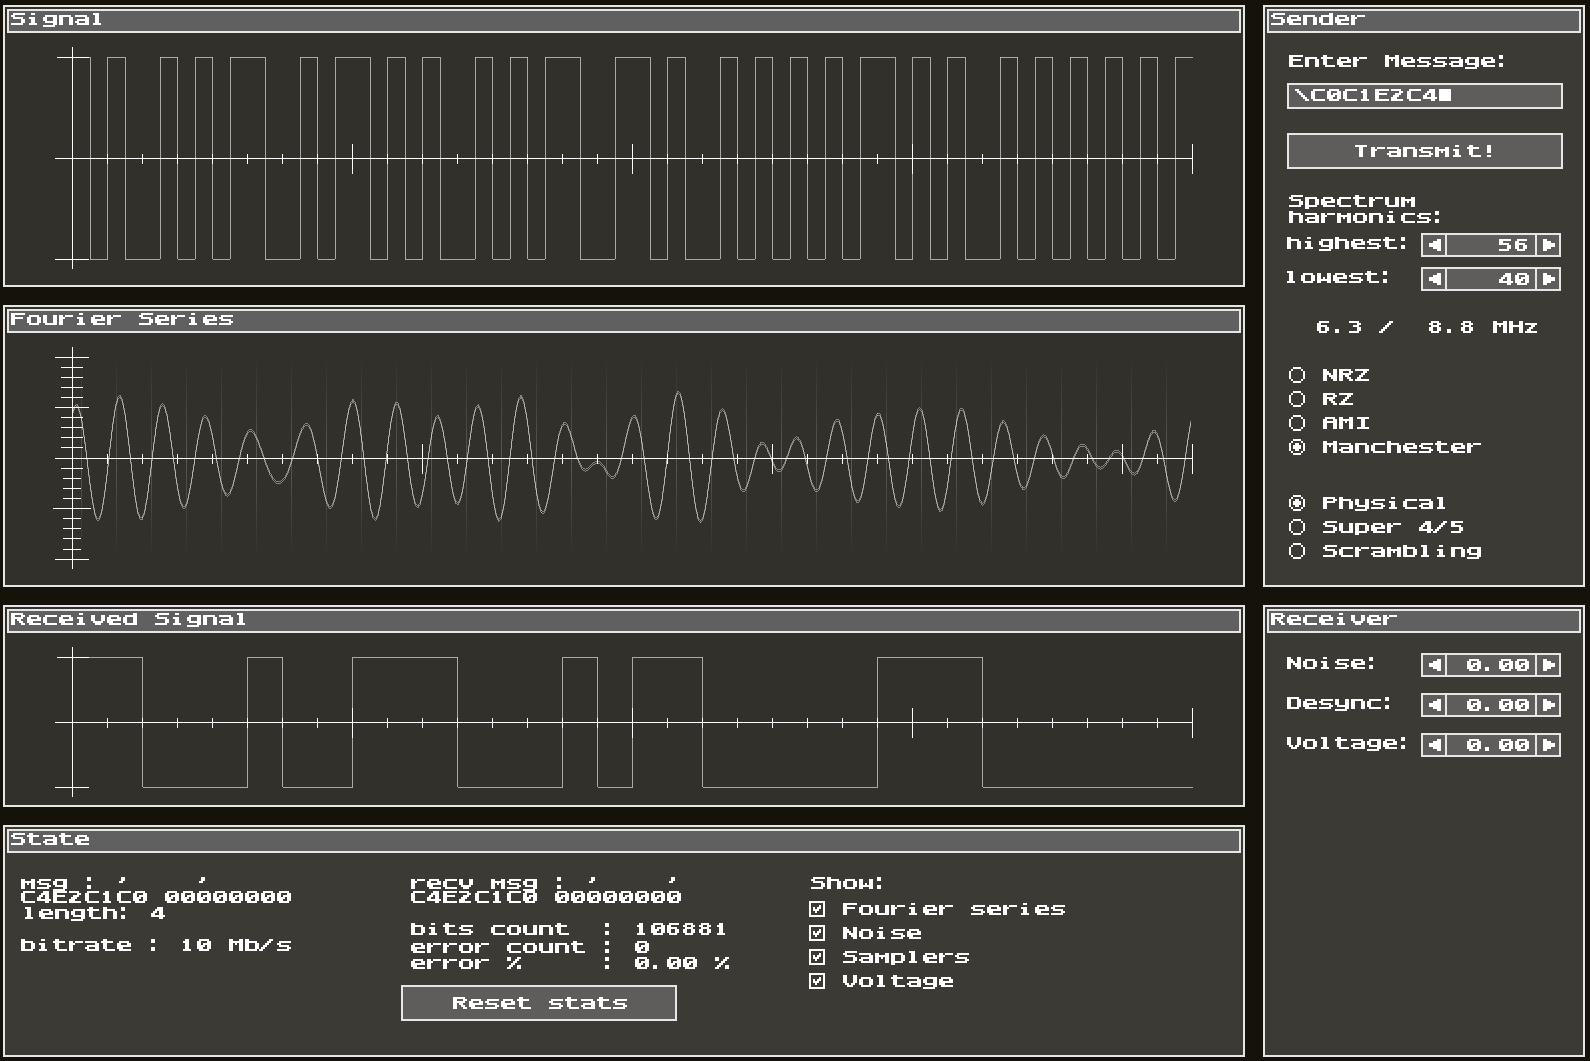
\includegraphics[width=0.95\linewidth]{./data/ideal_m2_min_f.png}
	\cutpic{0.2cm}{17cm}{./data/desync_nrz.png}
	\caption{Максимально допустимый уровень рассинхрона 0.35 для NRZ}
\end{figure}

\subsubsection{Voltage}

\begin{wrapfigure}{l}{0.7\textwidth}
	\centering
	% 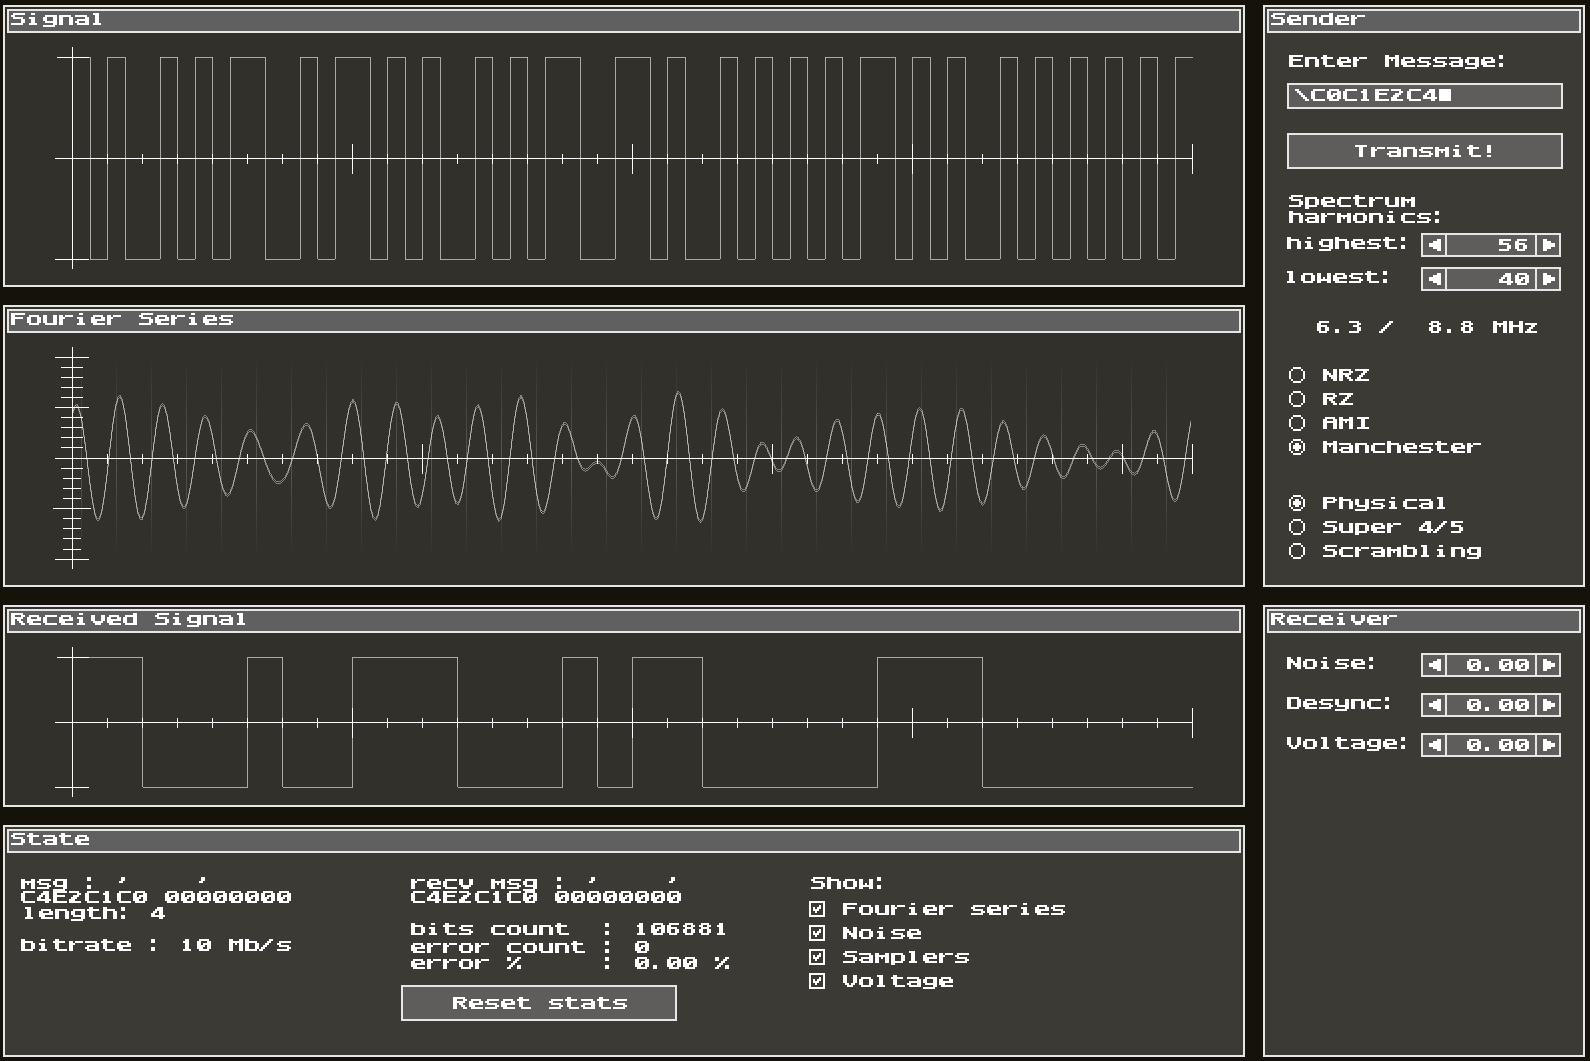
\includegraphics[width=0.95\linewidth]{./data/ideal_m2_min_f.png}
	\cutpic{0.2cm}{12cm}{./data/voltage_nrz.png}
	\caption{Уровень напряжения 0.38 для NRZ}
	\vspace{-100pt}
\end{wrapfigure}

Максимально допустимый уровень напряжения был определён с помощью программы \textit{Network Fourier} и составил \textbf{0.38}. Это граничное значение, ниже которого мы не будем считывать сигнал.


% ------------------------------------------------


\subsection{RZ}

\subsubsection{Noise}

Максимально допустимый уровень шума был определён с помощью программы \textit{Network Fourier} и составил \textbf{0.02}. Это граничное значение, при котором сигнал не искажается при воздействии произвольных гармоник.

\vspace{0.4cm}
\begin{figure}[h]
	\centering
	% 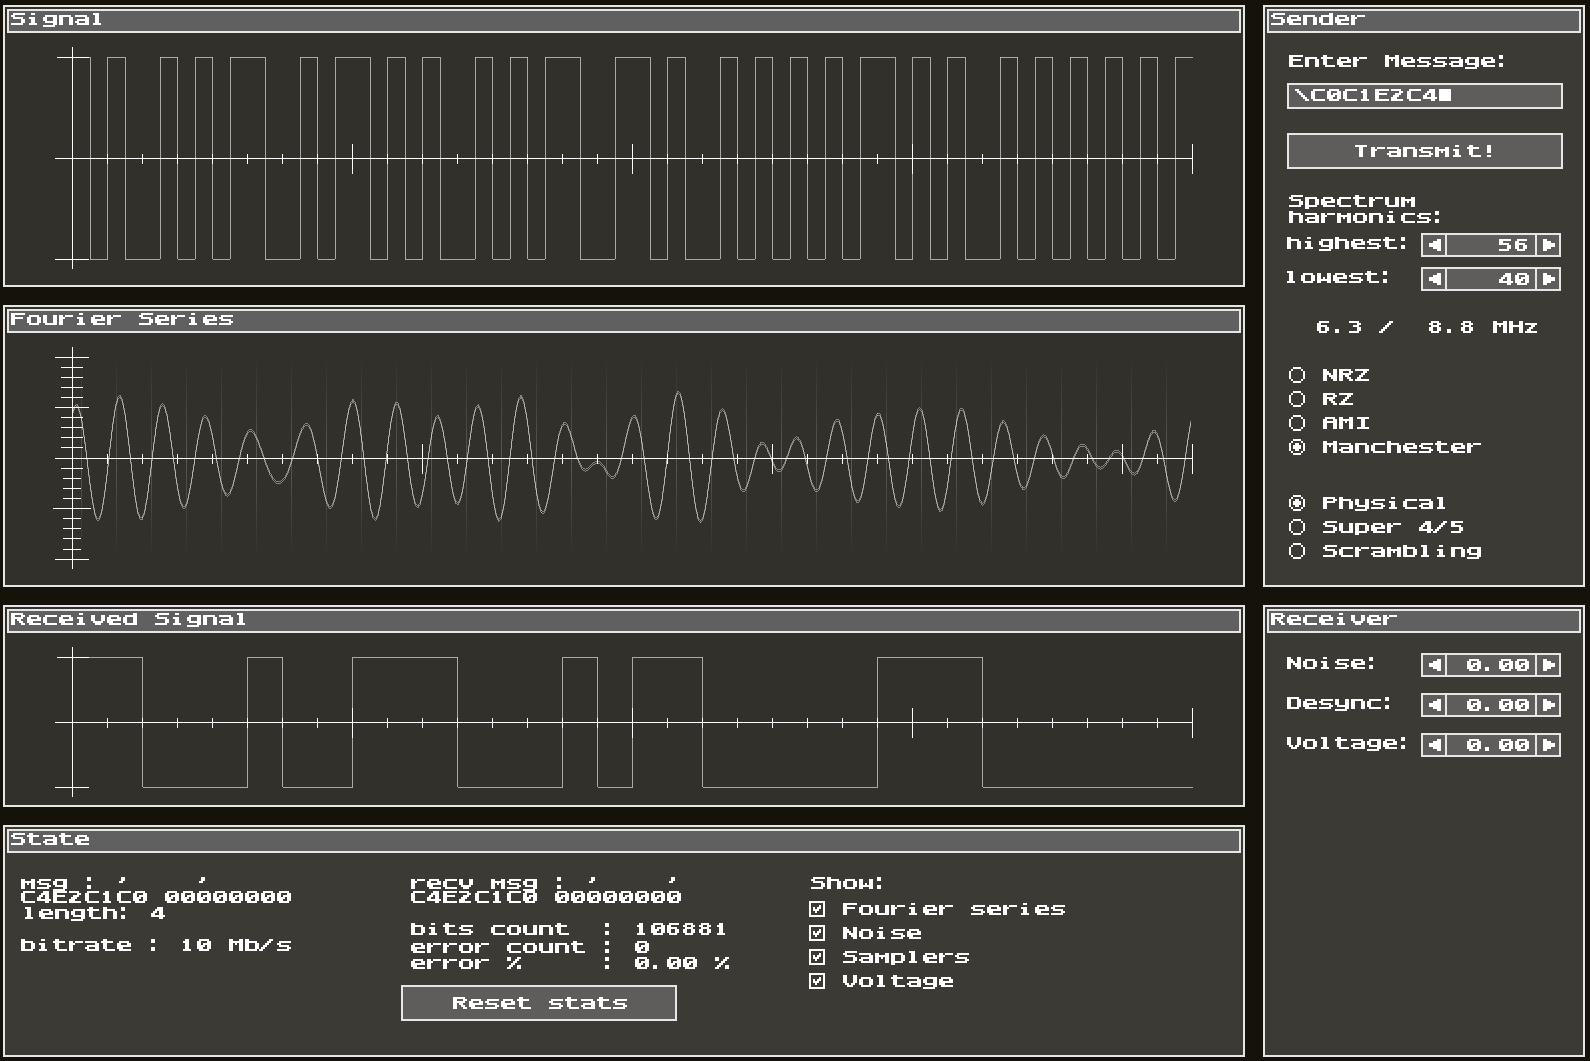
\includegraphics[width=0.95\linewidth]{./data/ideal_m2_min_f.png}
	\cutpic{0.2cm}{17cm}{./data/noise_rz.png}
	\caption{Максимально допустимый уровень шума 0.02 для RZ}
\end{figure}

\subsubsection{Desync}

\vspace{-0.2cm}
\begin{wrapfigure}{r}{0.65\textwidth}
	\centering
	% 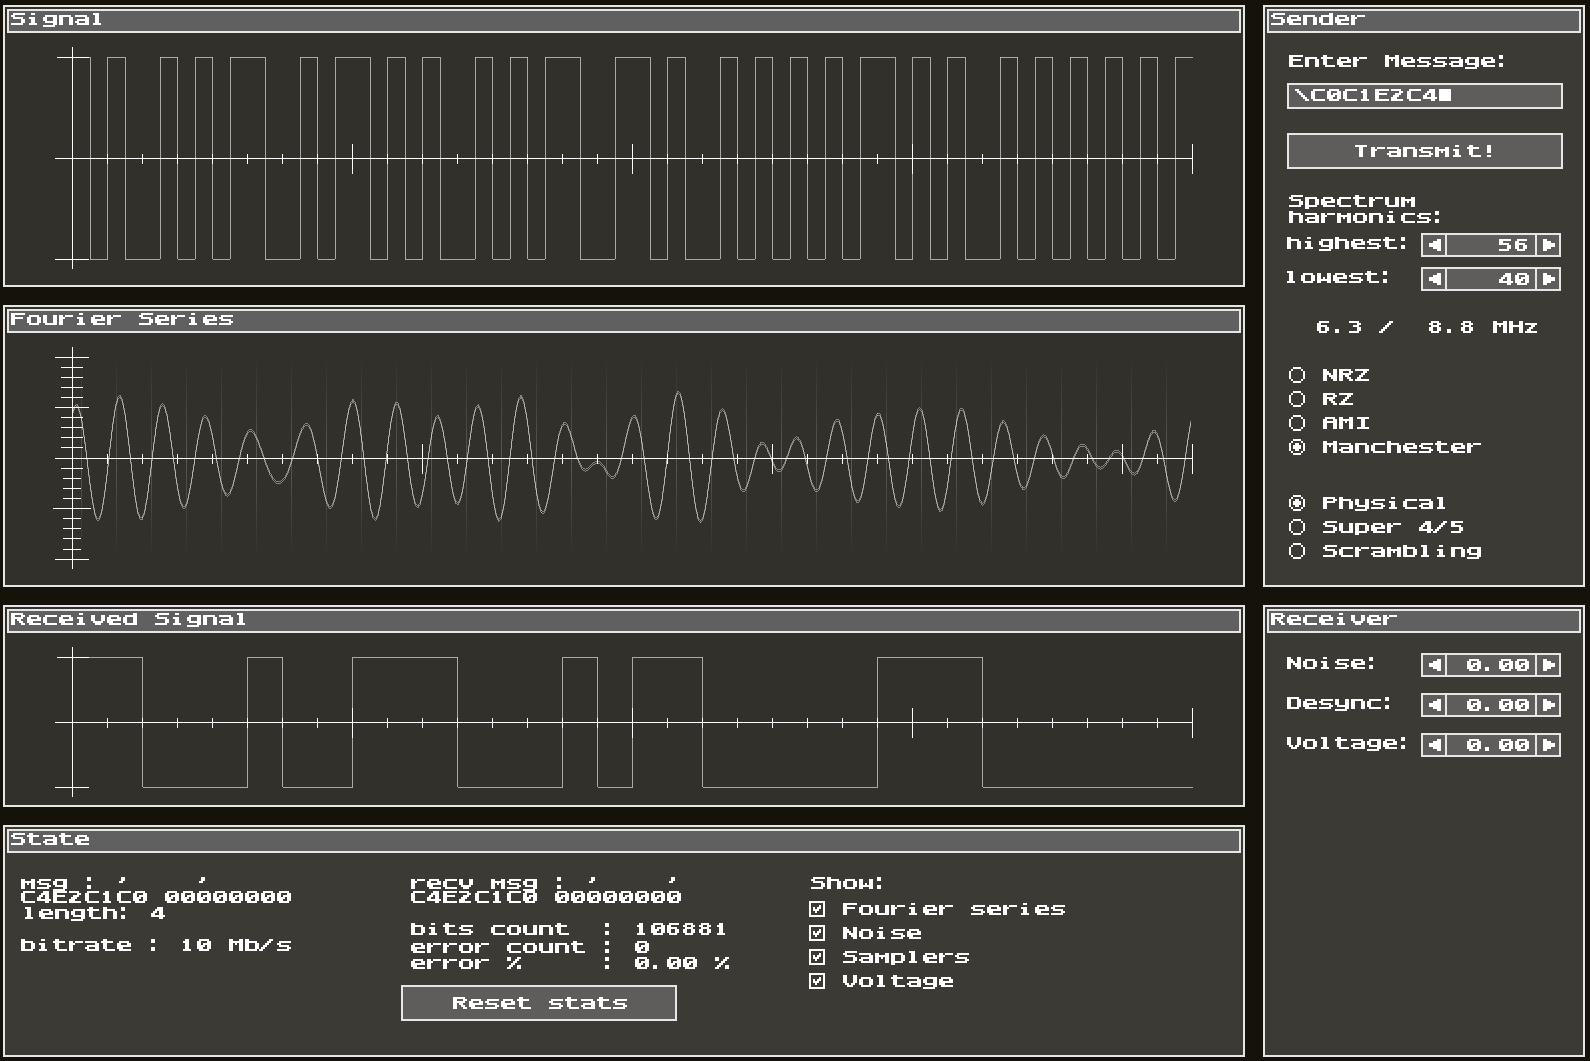
\includegraphics[width=0.95\linewidth]{./data/ideal_m2_min_f.png}
	\cutpic{0.2cm}{11.5cm}{./data/3_rz_desync.png.jpg}
	\caption{Уровень рассинхрона 0.02 для RZ}
	\vspace{-125pt}
\end{wrapfigure}

Максимально допустимый уровень рассинхронизации был определён с помощью программы \textit{Network Fourier} и составил \textbf{0.02}. Это граничное значение, при котором различие часов передатчика и приёмника не искажают сигнал.
\thispagestyle{empty}

\newpage

\subsubsection{Voltage}
Максимально допустимый уровень напряжения был определён с помощью программы \textit{Network Fourier} и составил \textbf{0.16}. Это граничное значение, ниже которого мы не будем считывать сигнал.

\vspace{0.4cm}
\begin{figure}[h]
	\centering
	% 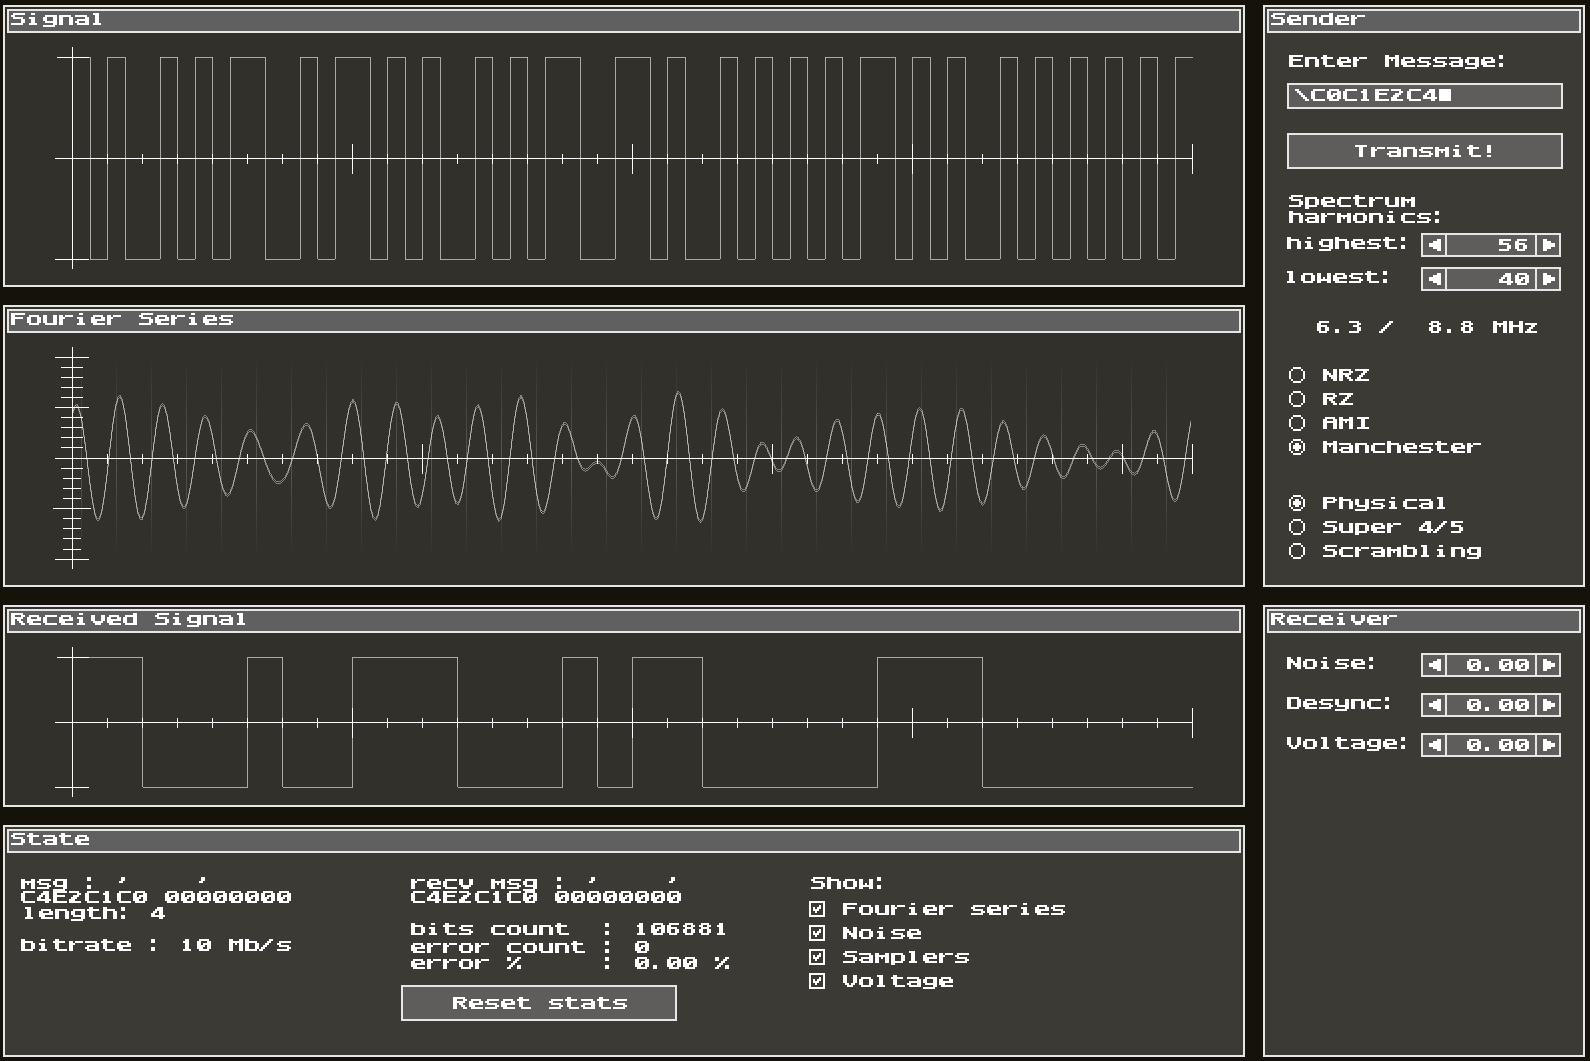
\includegraphics[width=0.95\linewidth]{./data/ideal_m2_min_f.png}
	\cutpic{0.2cm}{15cm}{./data/3_rz_voltage.png.jpg}
	\caption{Максимально допустимый уровень напряжения 0.16 для RZ}
\end{figure}


% ------------------------------------------------


\subsection{M2}

\subsubsection{Noise}

\vspace{-0.2cm}
\begin{wrapfigure}{r}{0.65\textwidth}
    \centering
    \cutpic{0.2cm}{11.5cm}{./data/3_m2_noise.png.jpg}
    \caption{Уровень шума 0.16 для M2}
    \vspace{-5cm}
\end{wrapfigure}
\thispagestyle{empty}

Максимально допустимый уровень шума был определён с помощью программы \textit{Network Fourier} и составил \textbf{0.16}. Это граничное значение, при котором сигнал не искажается при воздействии произвольных гармоник.

\newpage

\subsubsection{Desync}

Максимально допустимый уровень рассинхронизации был определён с помощью программы \textit{Network Fourier} и составил \textbf{0.1}. Это граничное значение, при котором различие часов передатчика и приёмника не искажают сигнал.

\vspace{0.4cm}
\begin{figure}[h]
	\centering
	% 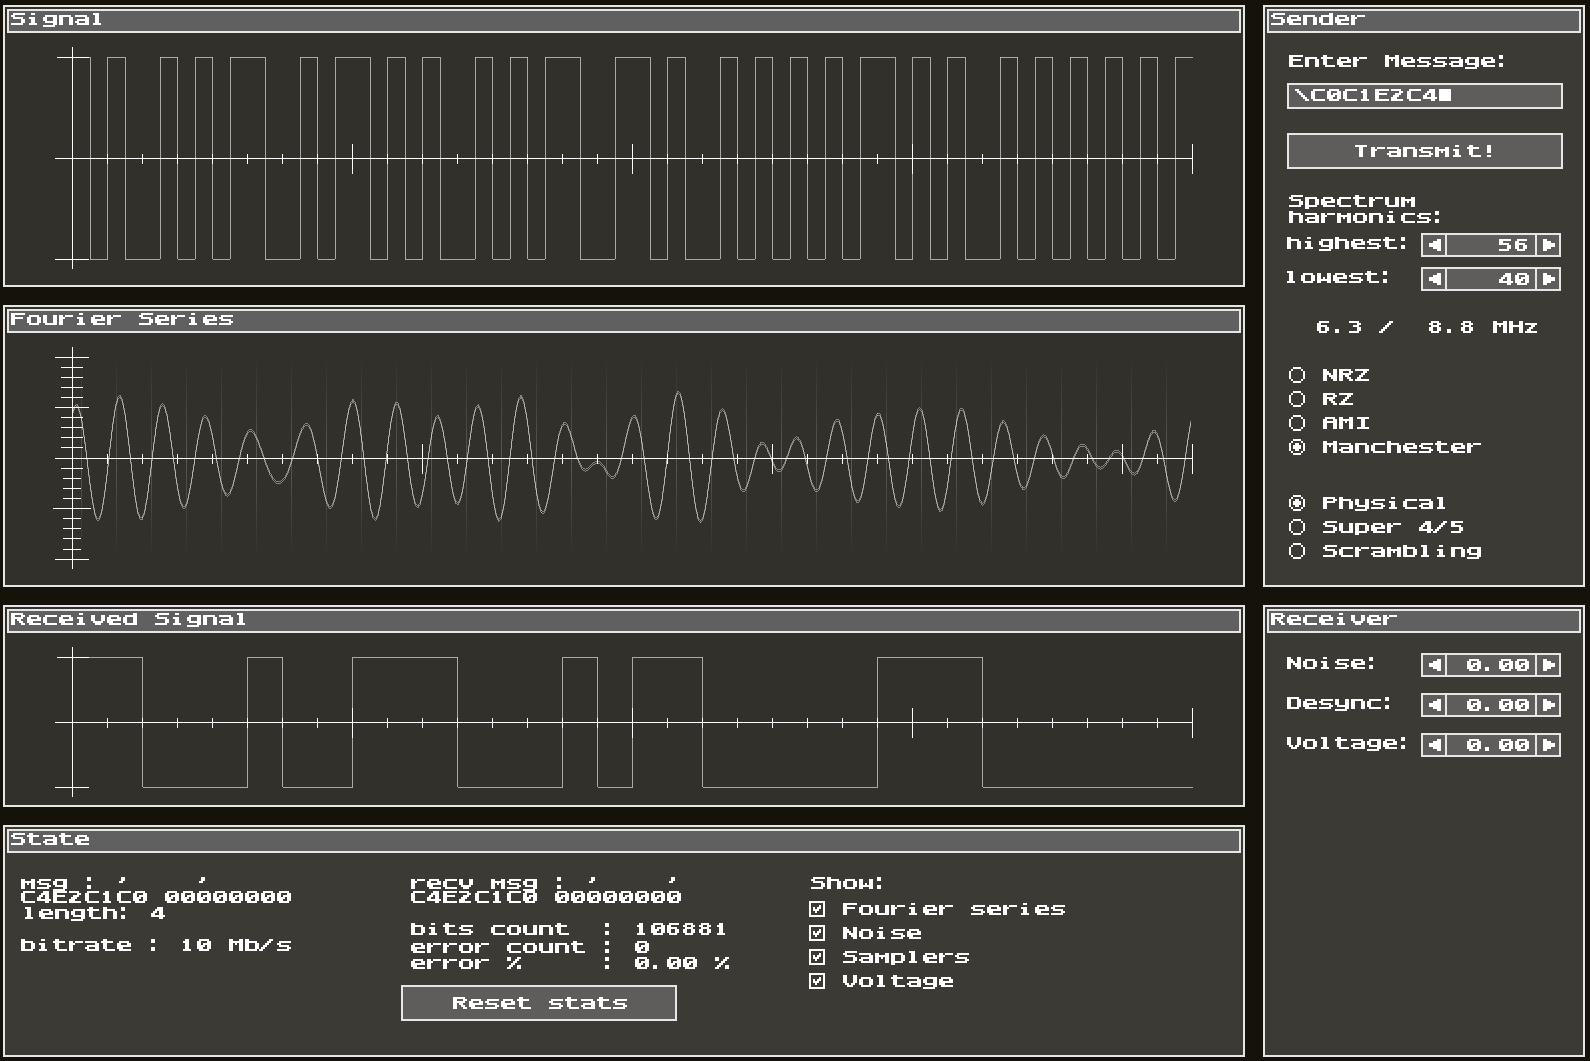
\includegraphics[width=0.95\linewidth]{./data/ideal_m2_min_f.png}
	\cutpic{0.2cm}{11.2cm}{./data/3_m2_desync.png.jpg}
	\caption{Максимально допустимый уровень рассинхронизации 0.1 для M2}
\end{figure}

\subsubsection{Voltage}

Максимально допустимый уровень напряжения был определён с помощью программы \textit{Network Fourier} и составил \textbf{0.1}. Это граничное значение, ниже которого мы не будем считывать сигнал.

\vspace{0.4cm}
\begin{figure}[h]
	\centering
	% 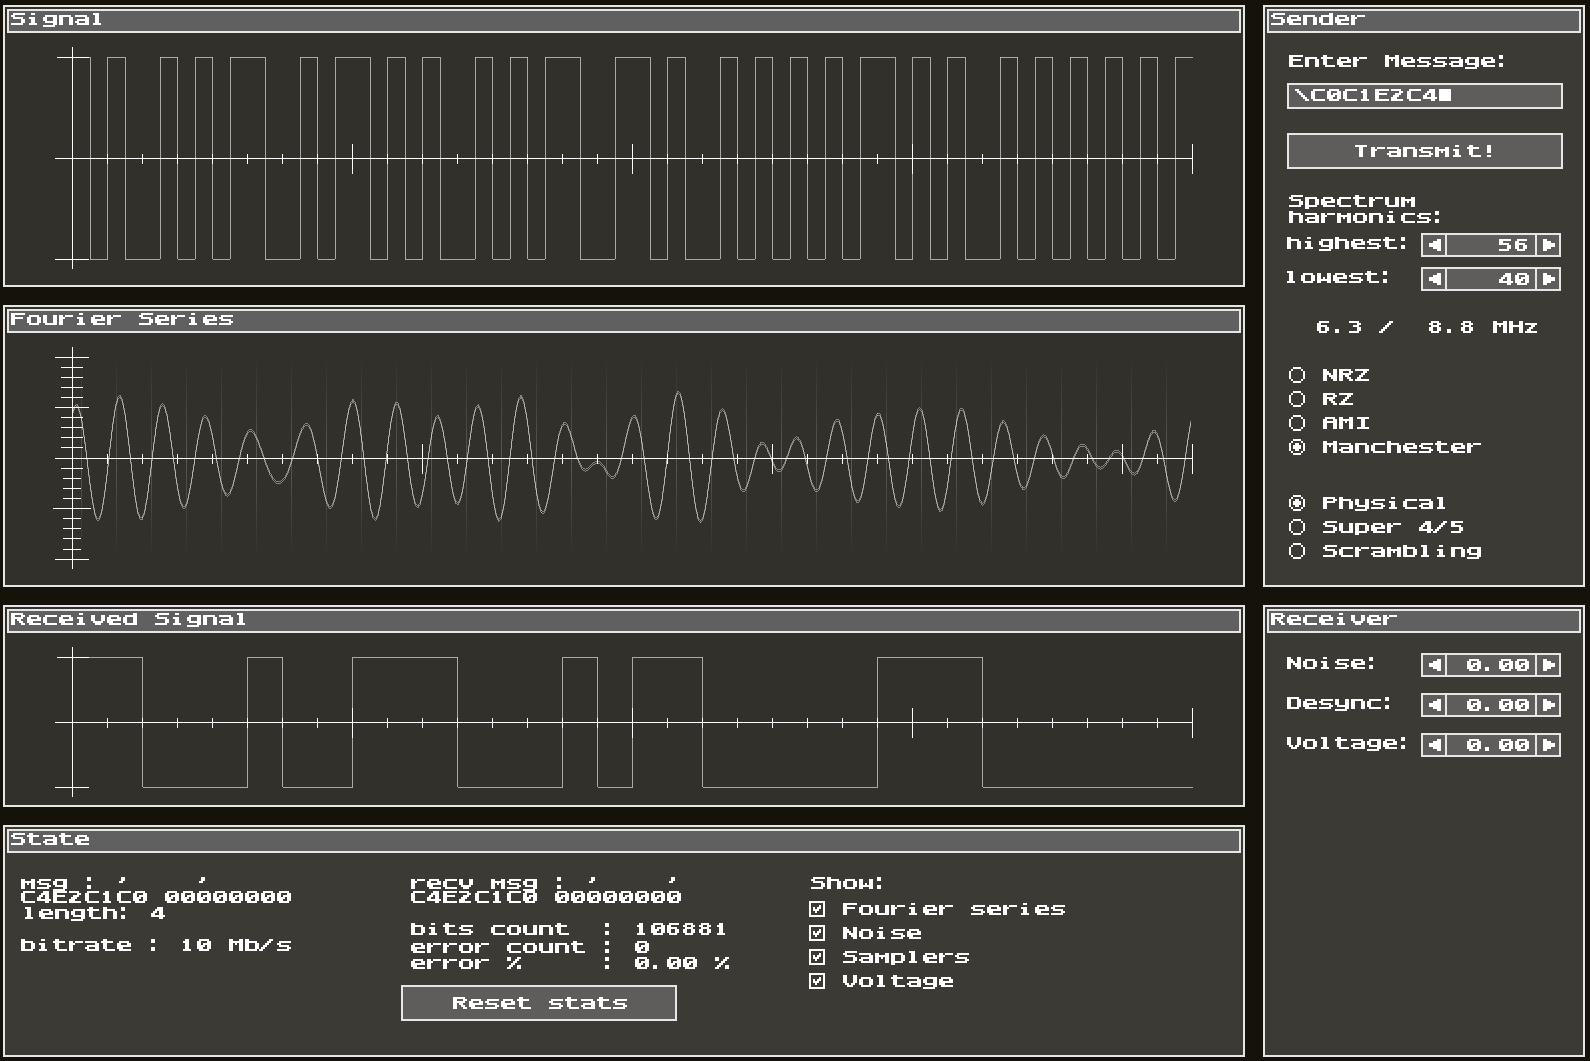
\includegraphics[width=0.95\linewidth]{./data/ideal_m2_min_f.png}
	\cutpic{0.2cm}{11.5cm}{./data/3_m2_voltage.png.jpg}
	\caption{Максимально допустимый уровень напряжения 1 для M2}
\end{figure}


% ------------------------------------------------


\newpage
\subsection{NRZ + 4B/5B}

\subsubsection{Noise}

Максимально допустимый уровень шума был определён с помощью программы \textit{Network Fourier} и составил \textbf{0.02}. Это граничное значение, при котором сигнал не искажается при воздействии произвольных гармоник.

\vspace{0.4cm}
\begin{figure}[h]
	\centering
	% 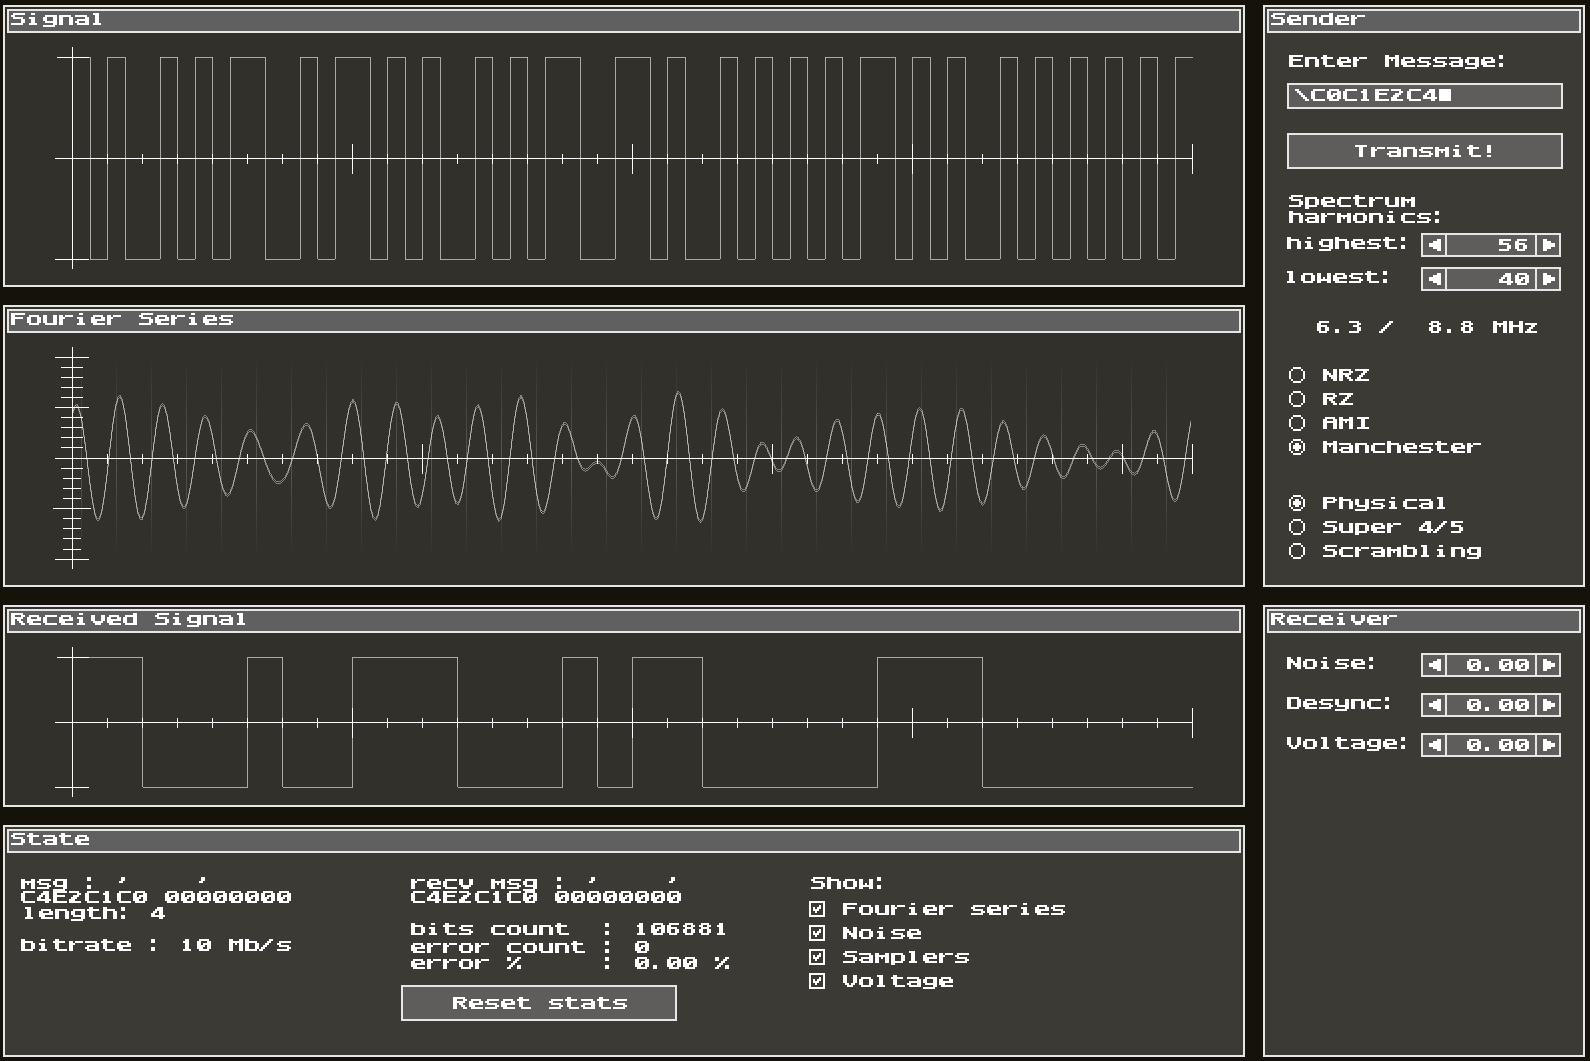
\includegraphics[width=0.95\linewidth]{./data/ideal_m2_min_f.png}
	\cutpic{0.2cm}{15cm}{./data/3_nrz45_noise.png.jpg}
	\caption{Максимально допустимый уровень шума 0.02 для NRZ+4B/5B}
\end{figure}

\subsubsection{Desync}

\vspace{-0.2cm}
\begin{wrapfigure}{r}{0.65\textwidth}
	\centering
	% 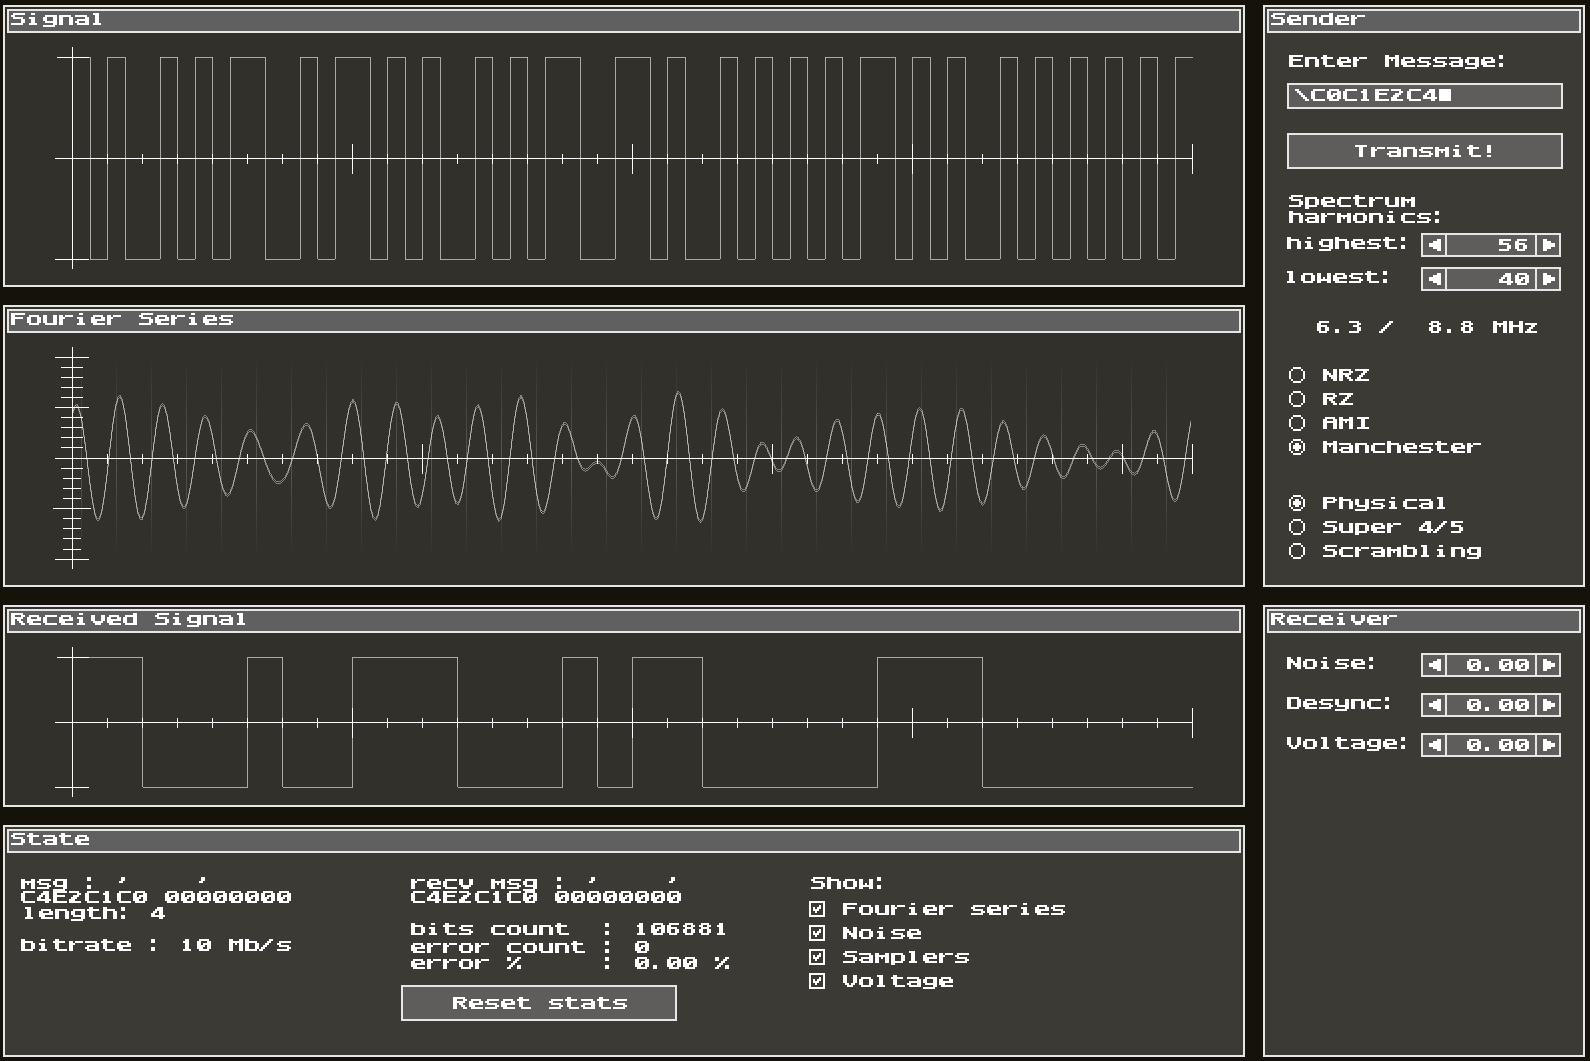
\includegraphics[width=0.95\linewidth]{./data/ideal_m2_min_f.png}
	\cutpic{0.2cm}{11.5cm}{./data/3_nrz45_desync.png.jpg}
	\caption{Уровень рассинхрона 0.12 для NRZ+4B/5B}
	\vspace{-125pt}
\end{wrapfigure}

Максимально допустимый уровень рассинхронизации был определён с помощью программы \textit{Network Fourier} и составил \textbf{0.12}. Это граничное значение, при котором различие часов передатчика и приёмника не искажают сигнал.
\thispagestyle{empty}

\newpage

\subsubsection{Voltage}
Максимально допустимый уровень напряжения был определён с помощью программы \textit{Network Fourier} и составил \textbf{0.02}. Это граничное значение, ниже которого мы не будем считывать сигнал.

\vspace{0.4cm}
\begin{figure}[h]
	\centering
	% 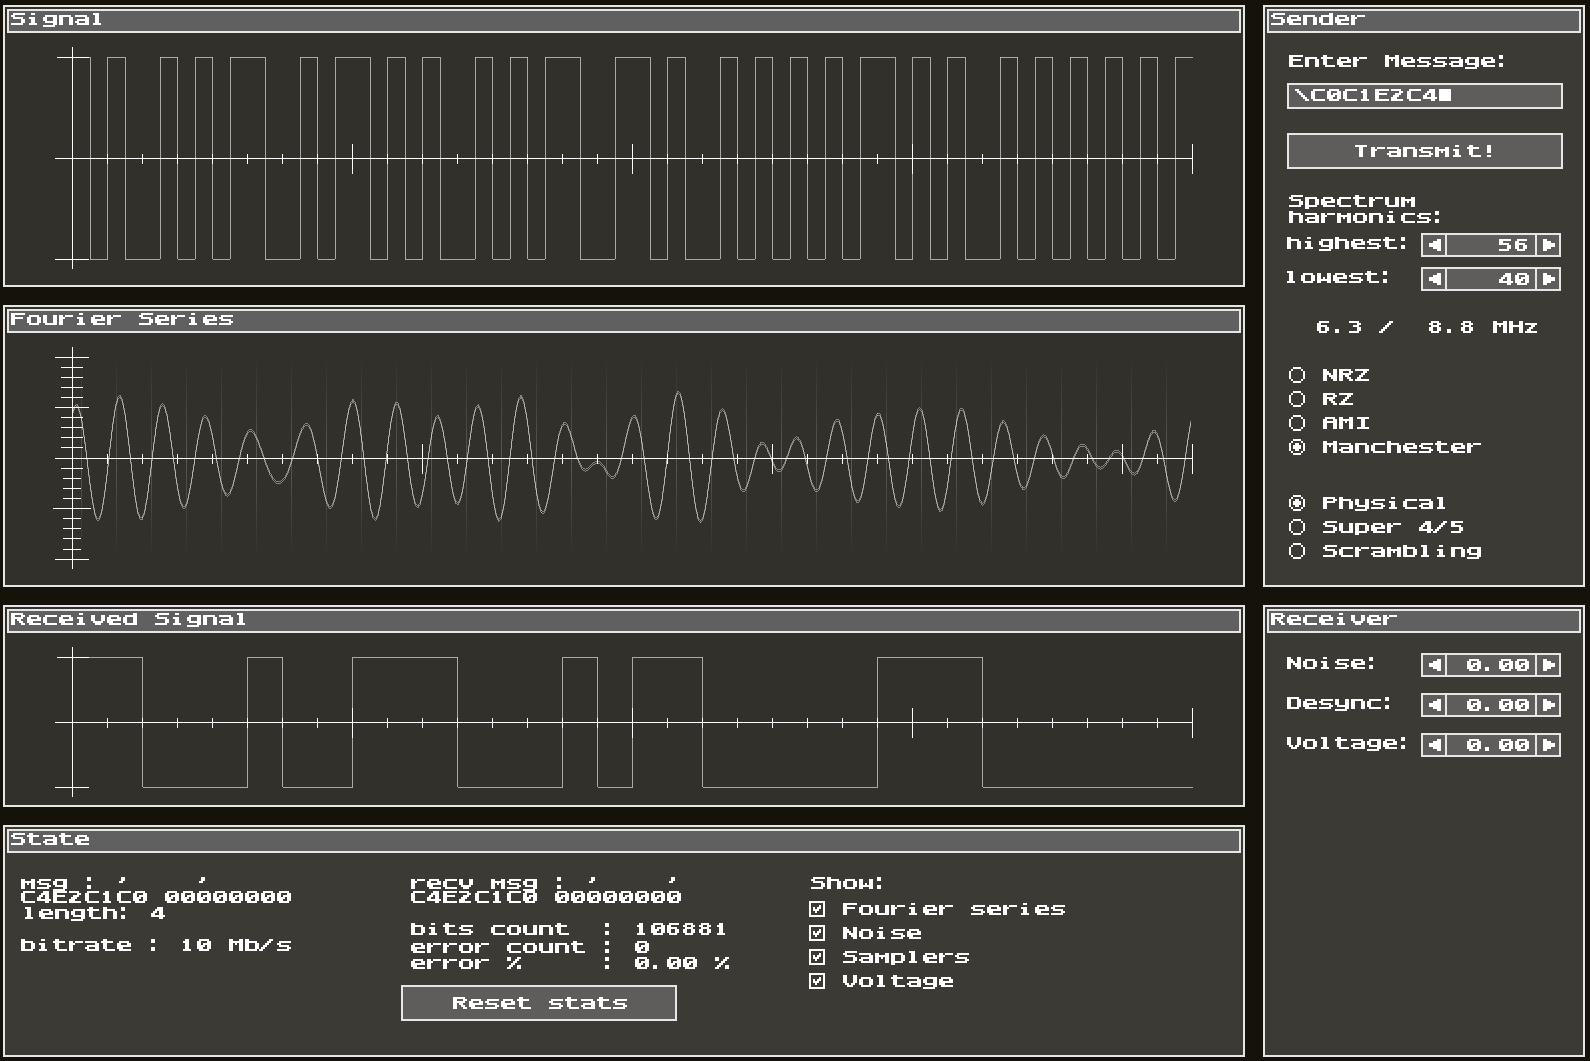
\includegraphics[width=0.95\linewidth]{./data/ideal_m2_min_f.png}
	\cutpic{0.2cm}{15cm}{./data/3_nrz45_voltage.png.jpg}
	\caption{Максимально допустимый уровень напряжения 0.02 для NRZ+4B/5B}
\end{figure}



% ------------------------------------------------


\subsection{NRZ + Scramble}

\subsubsection{Noise}

\vspace{-0.2cm}
\begin{wrapfigure}{r}{0.65\textwidth}
    \centering
    \cutpic{0.2cm}{11.5cm}{./data/3_nrzS_noise.png.jpg}
    \caption{Уровень шума 0.09 для NRZ + Scramble}
    \vspace{-5cm}
\end{wrapfigure}
\thispagestyle{empty}

Максимально допустимый уровень шума был определён с помощью программы \textit{Network Fourier} и составил \textbf{0.09}. Это граничное значение, при котором сигнал не искажается при воздействии произвольных гармоник.

\newpage

\subsubsection{Desync}

Максимально допустимый уровень рассинхронизации был определён с помощью программы \textit{Network Fourier} и составил \textbf{0.08}. Это граничное значение, при котором различие часов передатчика и приёмника не искажают сигнал.

\vspace{0.4cm}
\begin{figure}[h]
	\centering
	% 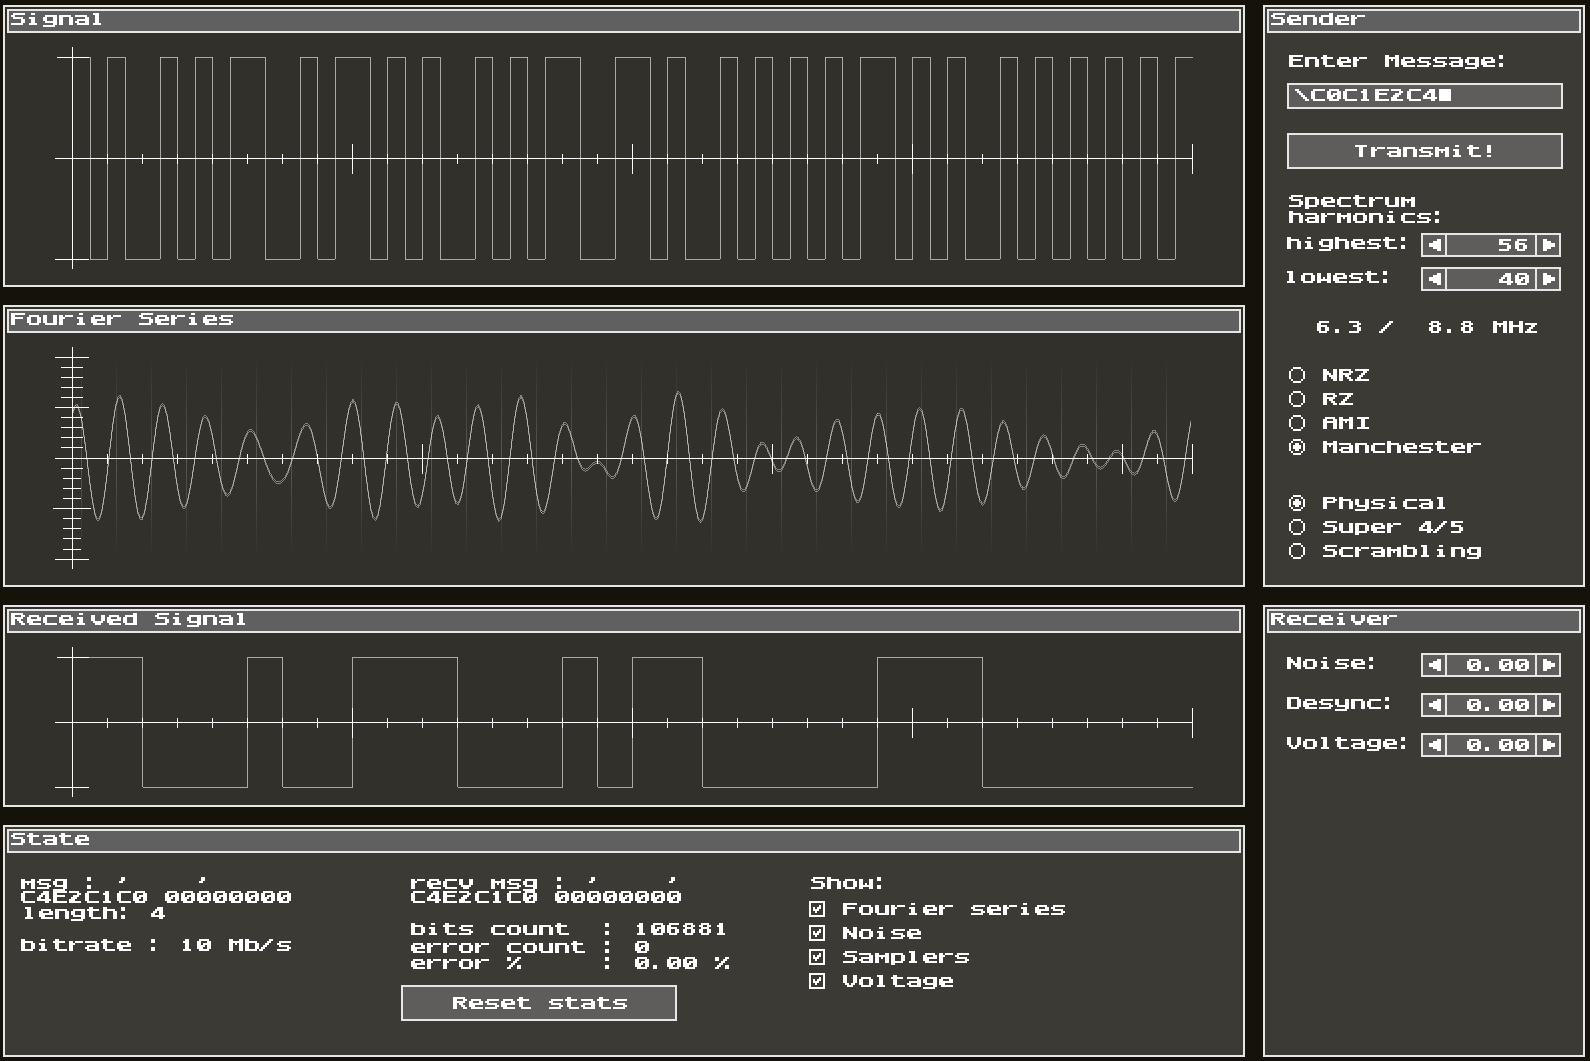
\includegraphics[width=0.95\linewidth]{./data/ideal_m2_min_f.png}
	\cutpic{0.2cm}{11.2cm}{./data/3_nrzS_desync.png.jpg}
	\caption{Макс. допустимый уровень рассинхрона 0.08 для NRZ+Scramble}
\end{figure}

\subsubsection{Voltage}

Максимально допустимый уровень напряжения был определён с помощью программы \textit{Network Fourier} и составил \textbf{0.37}. Это граничное значение, ниже которого мы не будем считывать сигнал.

\vspace{0.4cm}
\begin{figure}[h]
	\centering
	% 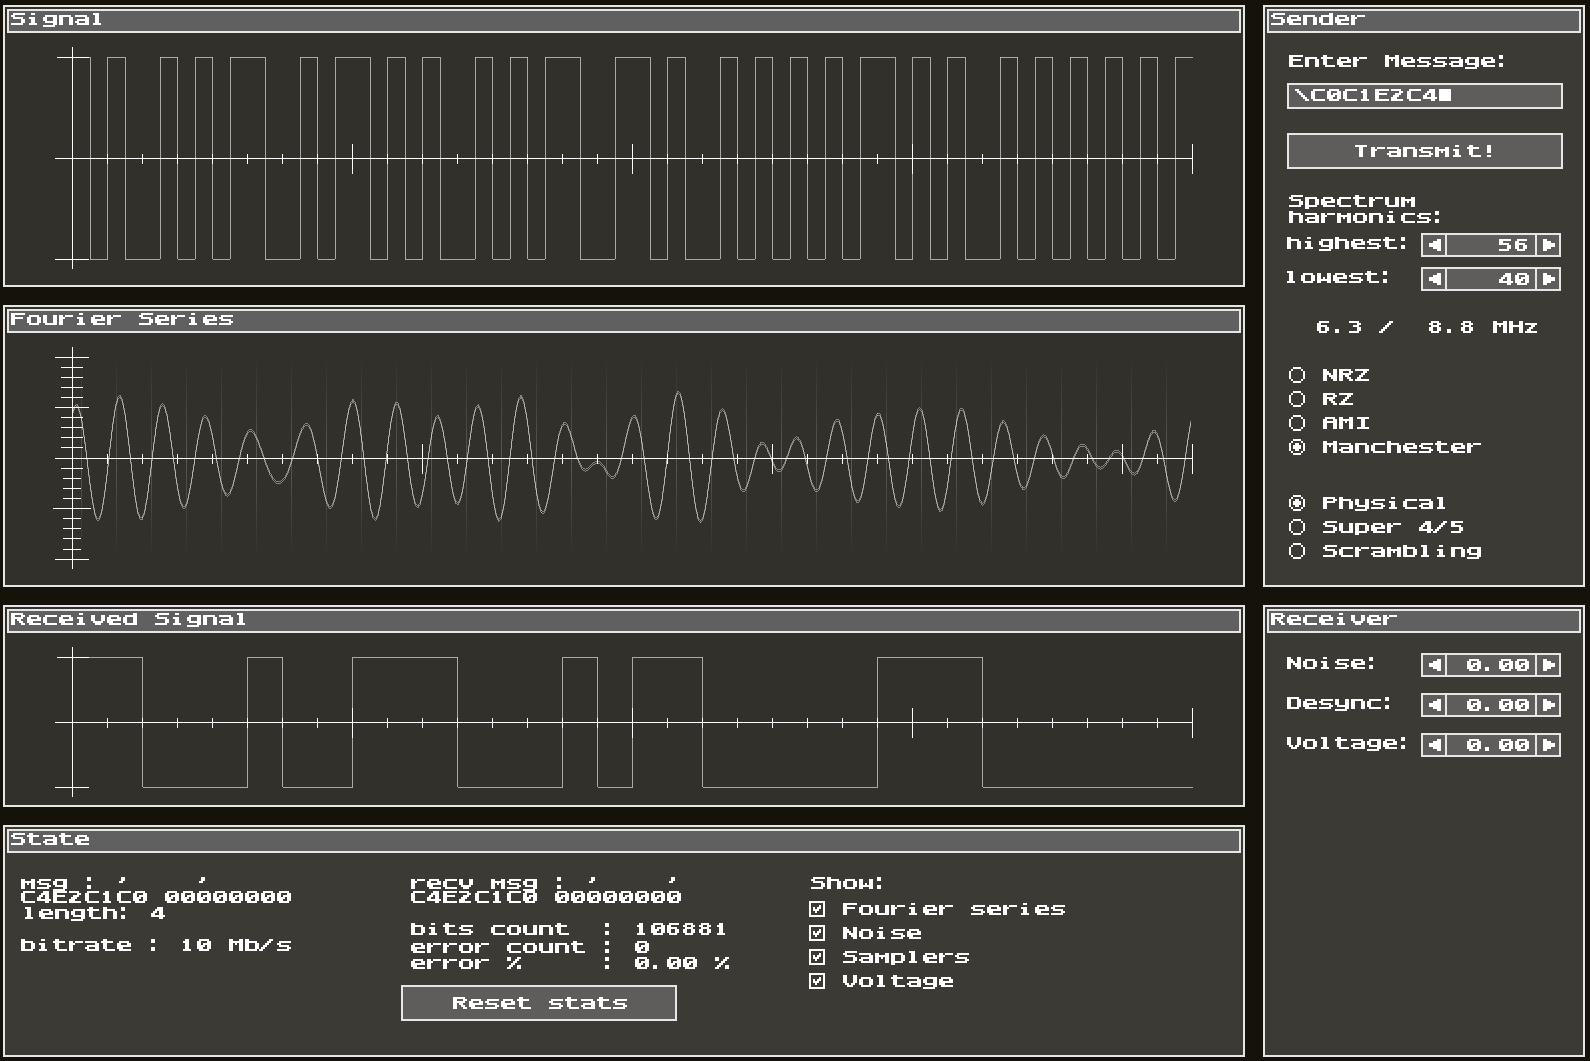
\includegraphics[width=0.95\linewidth]{./data/ideal_m2_min_f.png}
	\cutpic{0.2cm}{11.5cm}{./data/3_nrzS_voltage.png.jpg}
	\caption{Макс. допустимый уровень напряжения 0.37 для NRZ + Scramble}
\end{figure}


% ------------------------------------------------


\subsection{Выводы}

На данном этапе \underline{лучше остальных себя показали \textbf{NRZ} и \textbf{M2}}. 

У NRZ - лучшие показатели по уровню шума и рассинхронизации (0.2 и 0.35 соответственно), а уровень граничного шума (0.38) лучший после M2. Манчестер оказался невероятно устойчив к изменению уровня граничного напряжения до 1 В, что логично и объясняется тем, что он является импульсным кодом, и для его корректного приема неважен уровень напряжения, а важен переход напряжения от одного уровня к другому. Также, его уровень шума – на втором месте после NRZ (0.16), а уровень рассинхронизации (0.1) – на среднем уровне.

Худшие показатели у RZ (0.02, 0.02 и 0.16 при самой большой полосе пропускания). Этот метод показал себя хуже всех из-за необходимости обеспечения прочтения переходов сигнала в середине битового интервала в трех уровнях, что сложнее при ограниченной полосе пропускания, чем для двухуровневого M2, который также является импульсным.

NRZ+4B/5B и NRZ+Scramble показали результаты хуже чем сам NRZ. Такой результат обусловлен тем, что это потенциальные коды, и их плохая устойчивость к помехам обусловлена в том числе и содержанием сообщения, поэтому результаты по каждому из виду помех могут сильно отличаться друг от друга. Отметим только то, что NRZ+Scramble показал почти одинаковый уровень граничного напряжения (0.37) с NRZ (0.38), остальные параметры оказались хуже. А NRZ+4B/5B оказался хуже NRZ по всем параметрам.



% -------------------------------

\section{Достоверность распознавания сигналов на \-приеме}
На данном этапе я определил процент ошибок при передаче сообщения, используя найденные на предыдущем этапе максимально допустимые значения уровней шумов, рассинхронизации, граничного напряжения, и минимальную полосу пропускания канала связи.

\subsection{NRZ}

\begin{wrapfigure}{l}{0.65\textwidth}
	\centering
	% 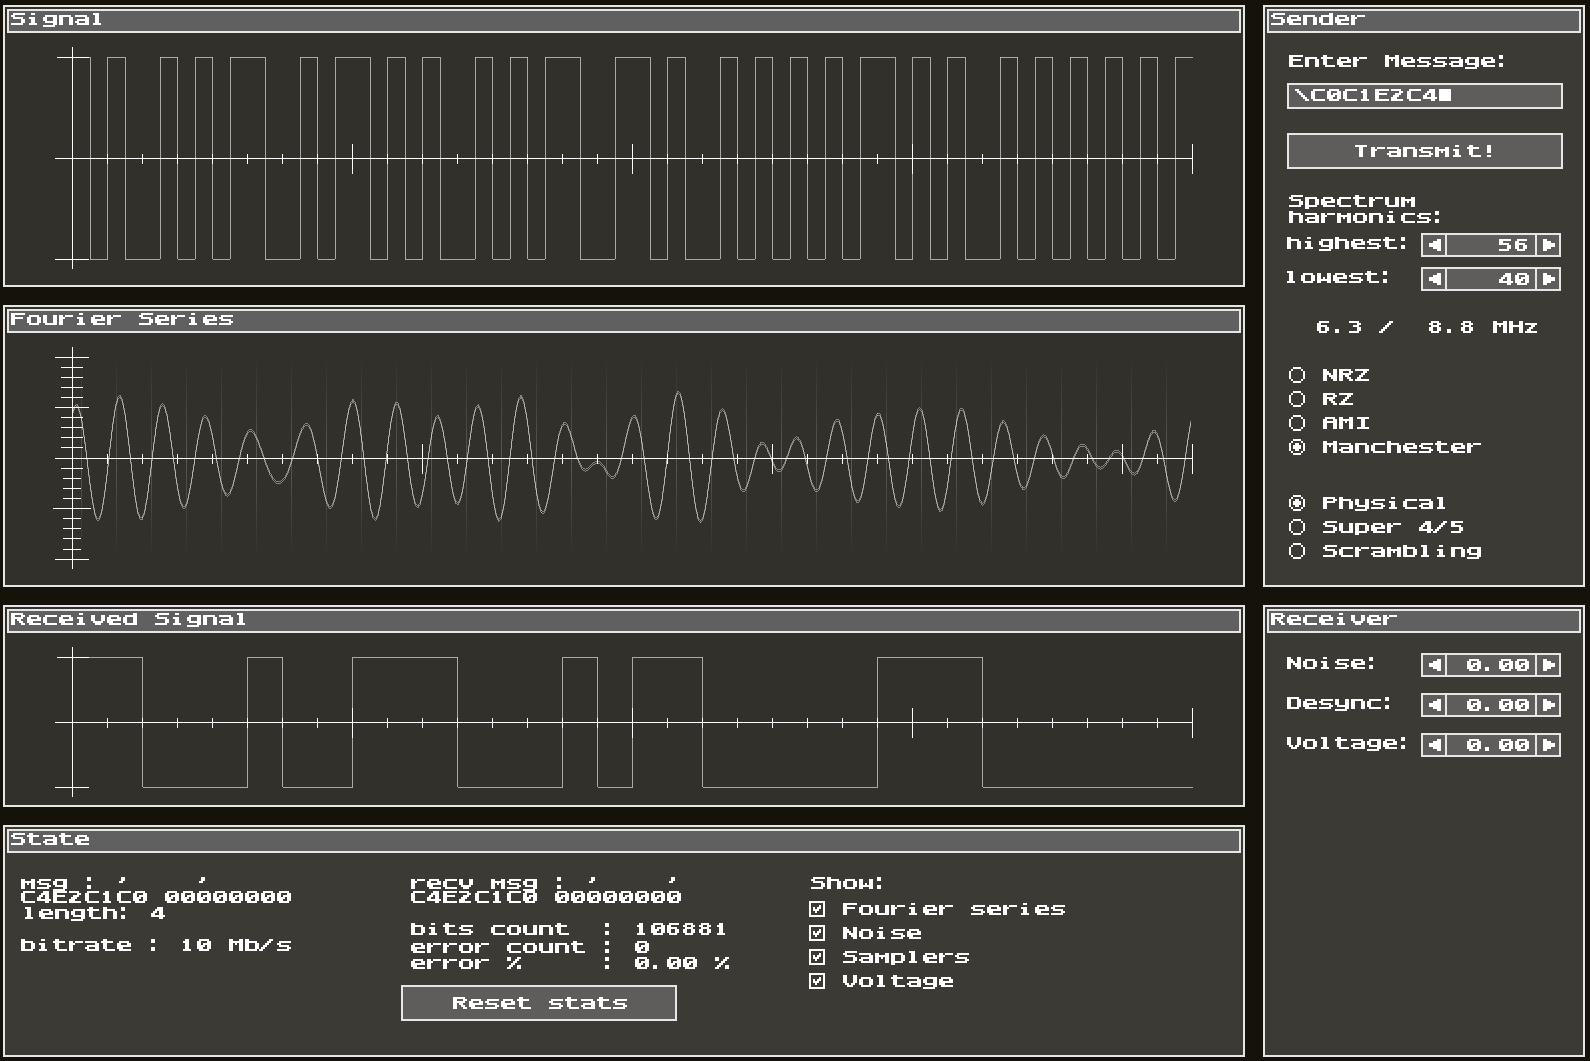
\includegraphics[width=0.95\linewidth]{./data/ideal_m2_min_f.png}
	\cutpic{0.2cm}{11cm}{./data/4_nrz.png.jpg}
	\caption{Процент ошибок для NRZ}
	\vspace{-115pt}
\end{wrapfigure}

Для NRZ при передаче 100000 бит при минимальной ширине полосы пропускания и максимально допустимых уровнях шума, рассинхронизации и граничного напряжения, процент ошибок составил 2.36\%.

\thispagestyle{empty}

\newpage

\subsection{RZ}

\vspace{0.4cm}
\begin{wrapfigure}{r}{0.6\textwidth}
	\centering
	% 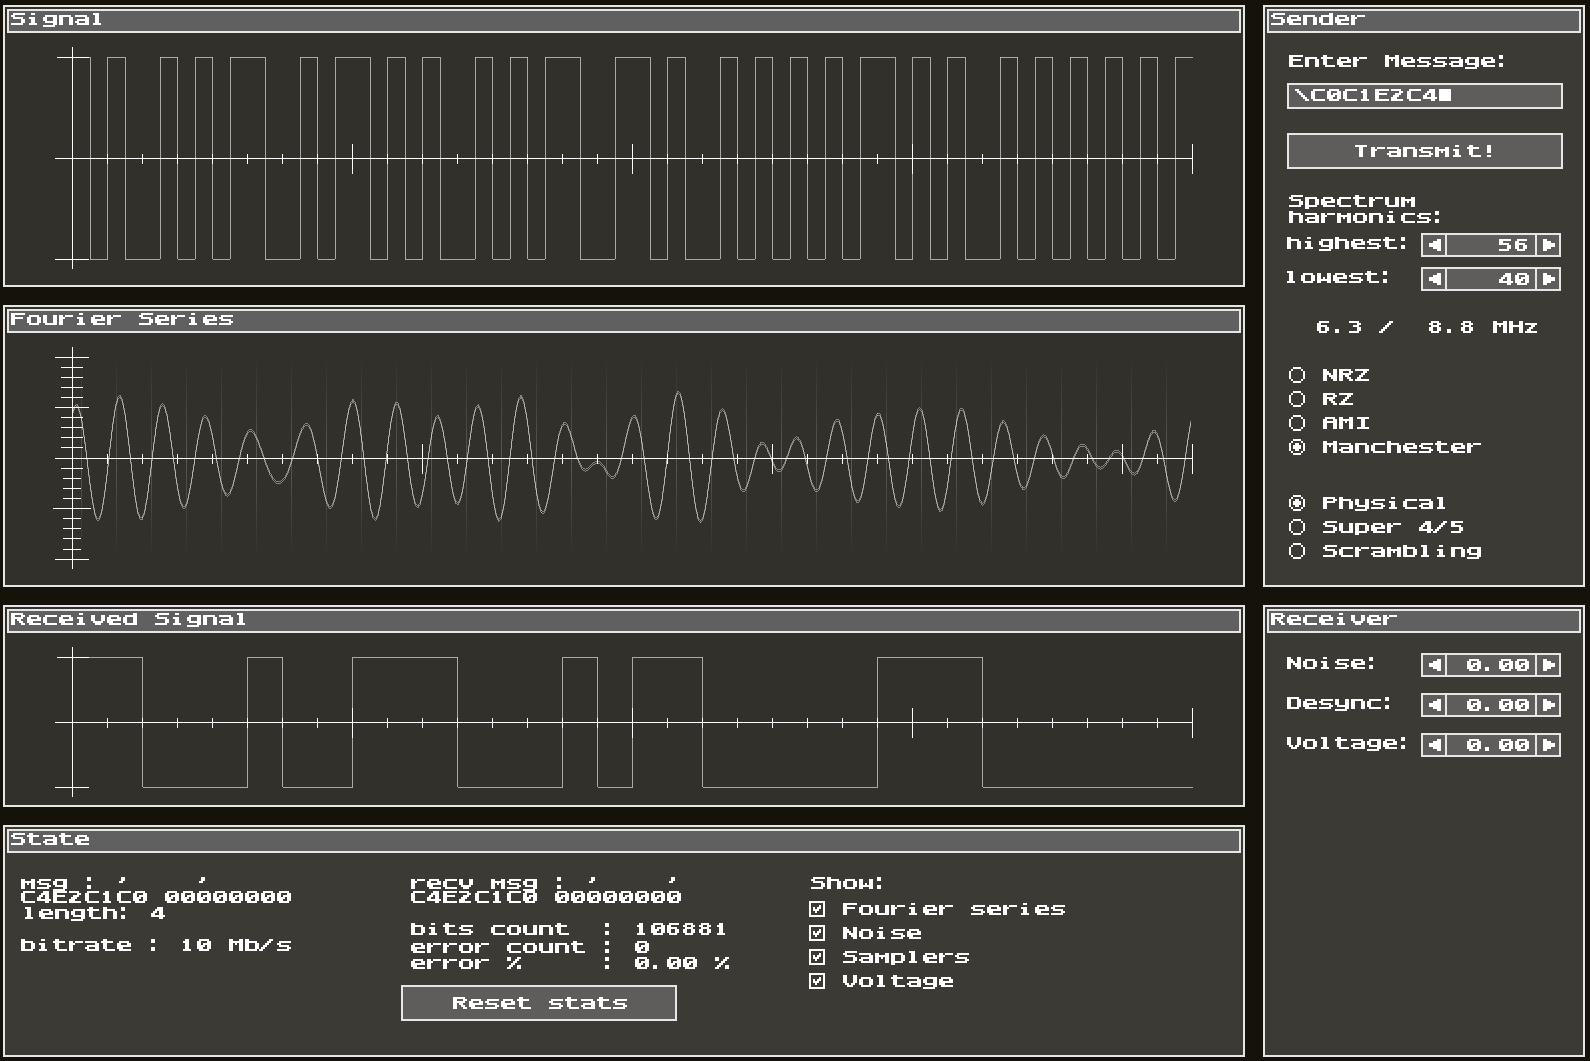
\includegraphics[width=0.95\linewidth]{./data/ideal_m2_min_f.png}
	\cutpic{0.2cm}{11.7cm}{./data/4_rz.png.jpg}
	\caption{Процент ошибок для RZ}
\end{wrapfigure}

Для RZ при передаче 100000 бит при минимальной ширине полосы пропускания и максимально допустимых уровнях шума, рассинхронизации и граничного напряжения, процент ошибок составил 1.2\%.

\subsection{M2}

Для M2 при передаче порядка 100000 бит при минимальной ширине полосы пропускания и максимально допустимых уровнях шума, рассинхронизации и граничного напряжения, процент ошибок составил 0.08\%.

\vspace{0.4cm}
\begin{figure}[H]
	\centering
	% 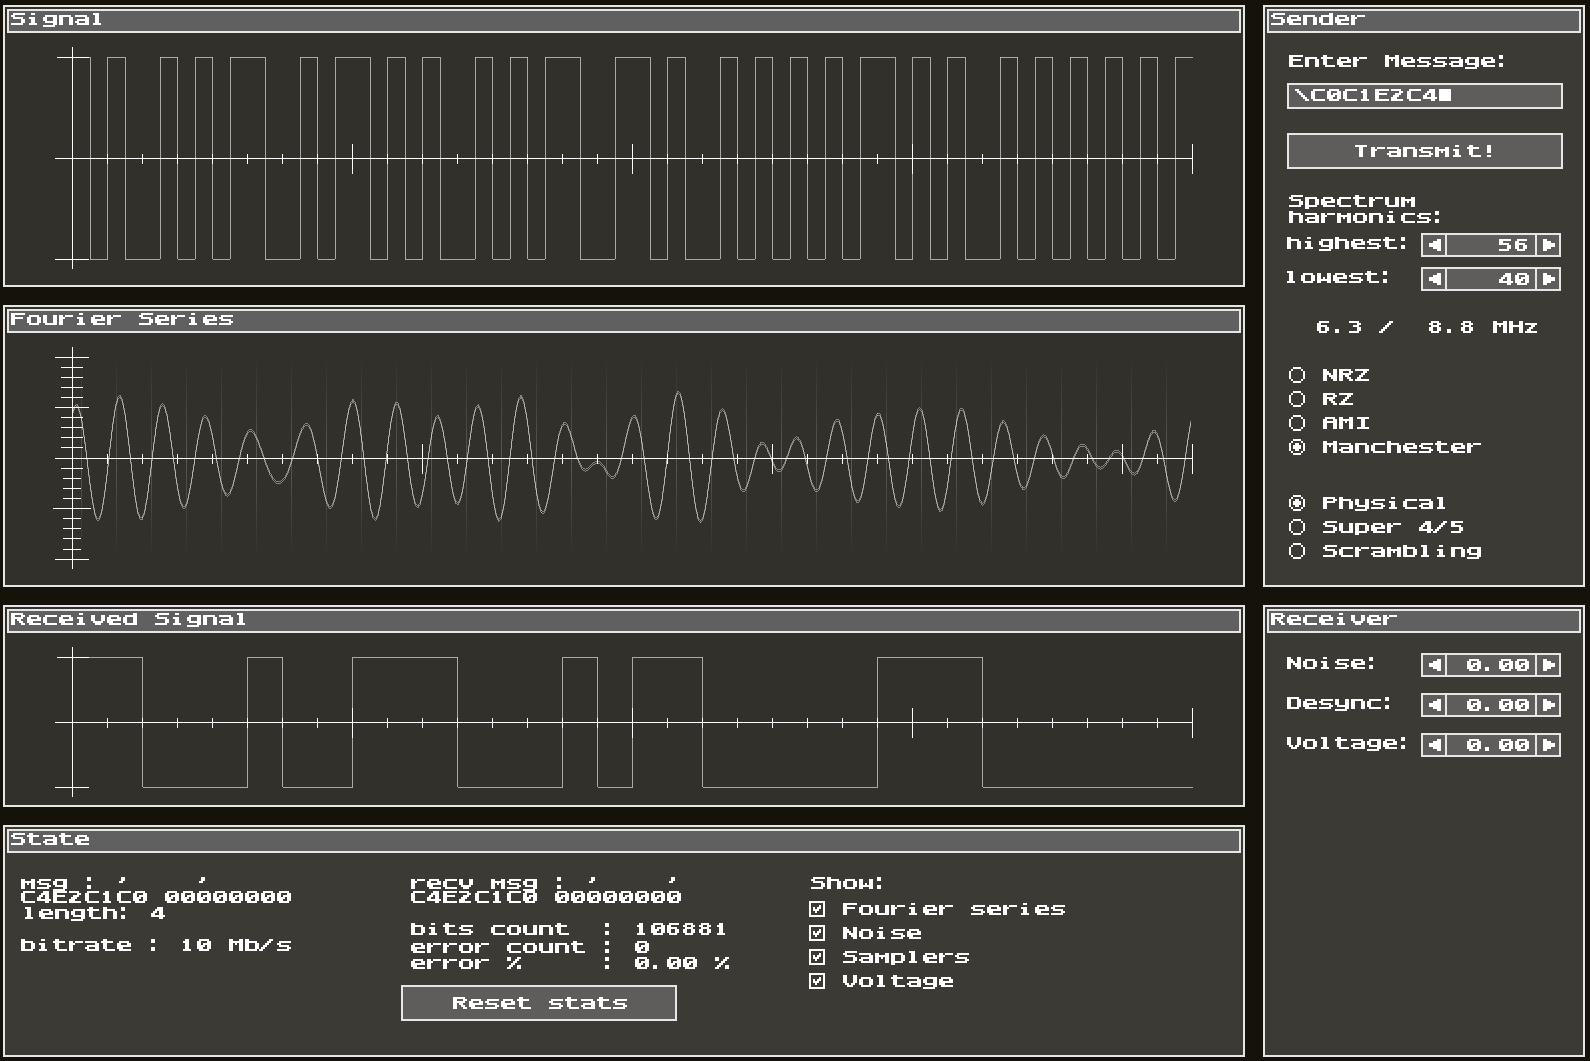
\includegraphics[width=0.95\linewidth]{./data/ideal_m2_min_f.png}
	\cutpic{0.2cm}{16.5cm}{./data/4_m2.png.jpg}
	\caption{Процент ошибок для M2}
\end{figure}

\subsection{NRZ + 4B/5B}

\vspace{0.4cm}
\begin{wrapfigure}{l}{0.7\textwidth}
	\centering
	% 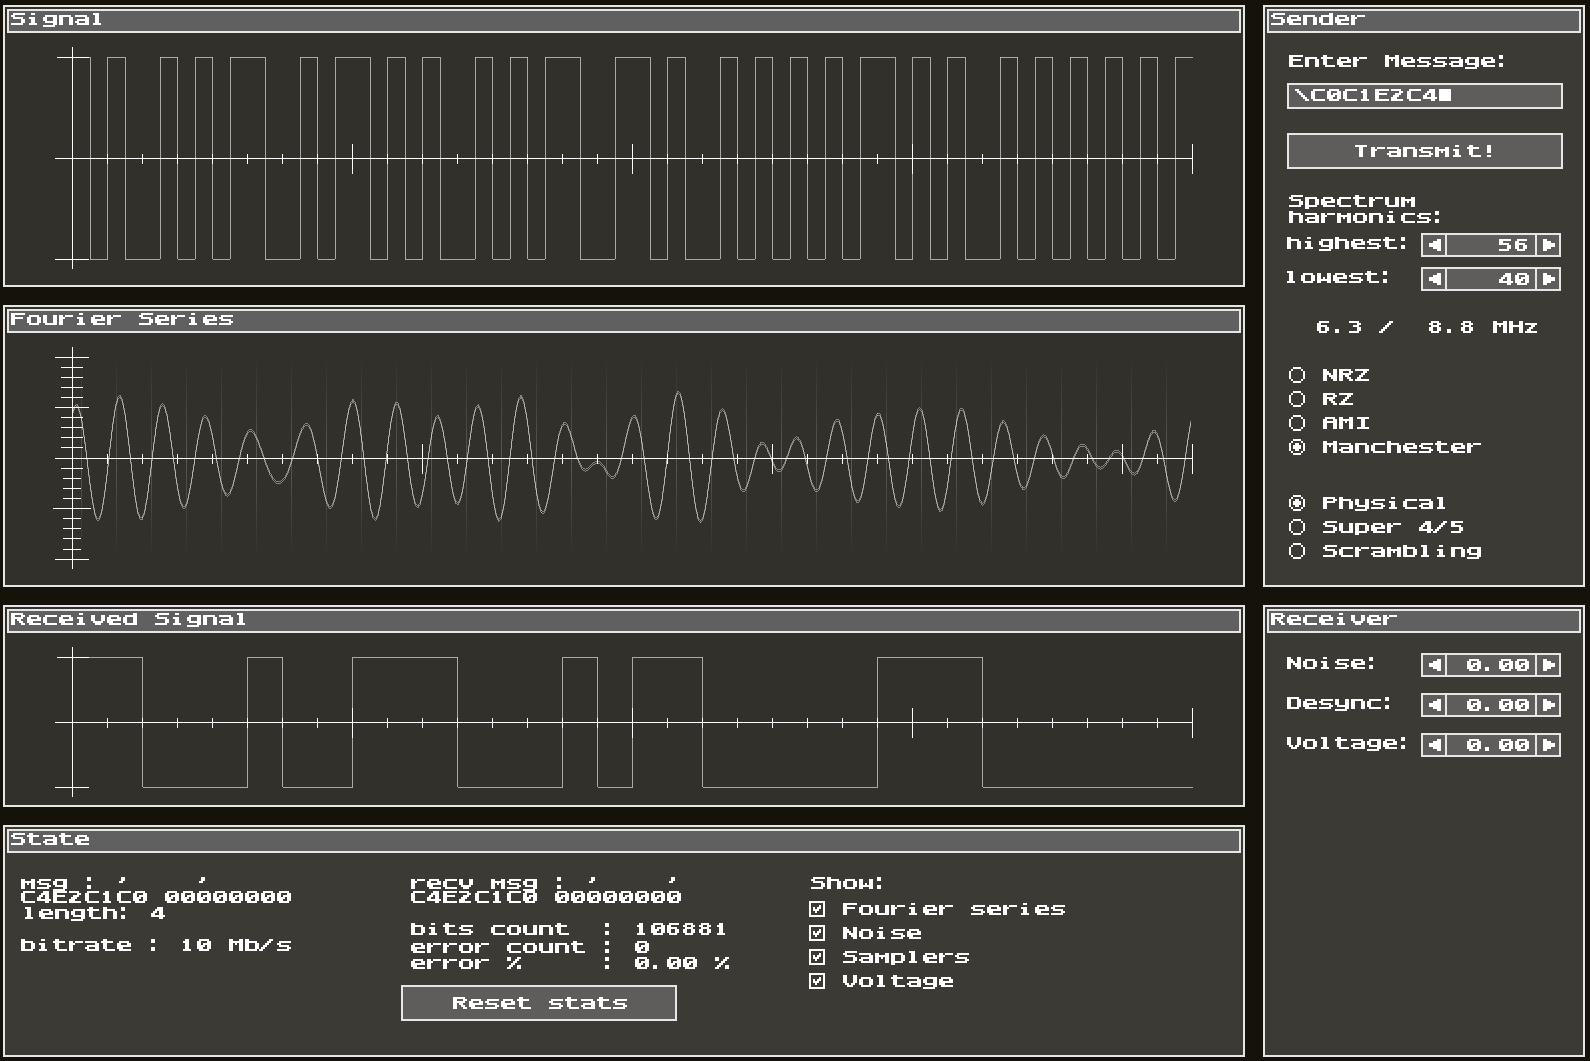
\includegraphics[width=0.95\linewidth]{./data/ideal_m2_min_f.png}
	\cutpic{0.2cm}{12cm}{./data/4_nrz45.png.jpg}
	\caption{Процент ошибок для NRZ + 4B/5B}
    \vspace{-3.7cm}
\end{wrapfigure}

Для NRZ+4B/5B при передаче порядка порядка 100000 бит при минимальной ширине полосы пропускания и максимально допустимых уровнях шума, рассинхронизации и граничного напряжения, процент ошибок составил 1.25\%.

\vspace{3.7cm}
\subsection{NRZ + Scramble}

\vspace{0.4cm}
\begin{wrapfigure}{r}{0.73\textwidth}
	\centering
	% 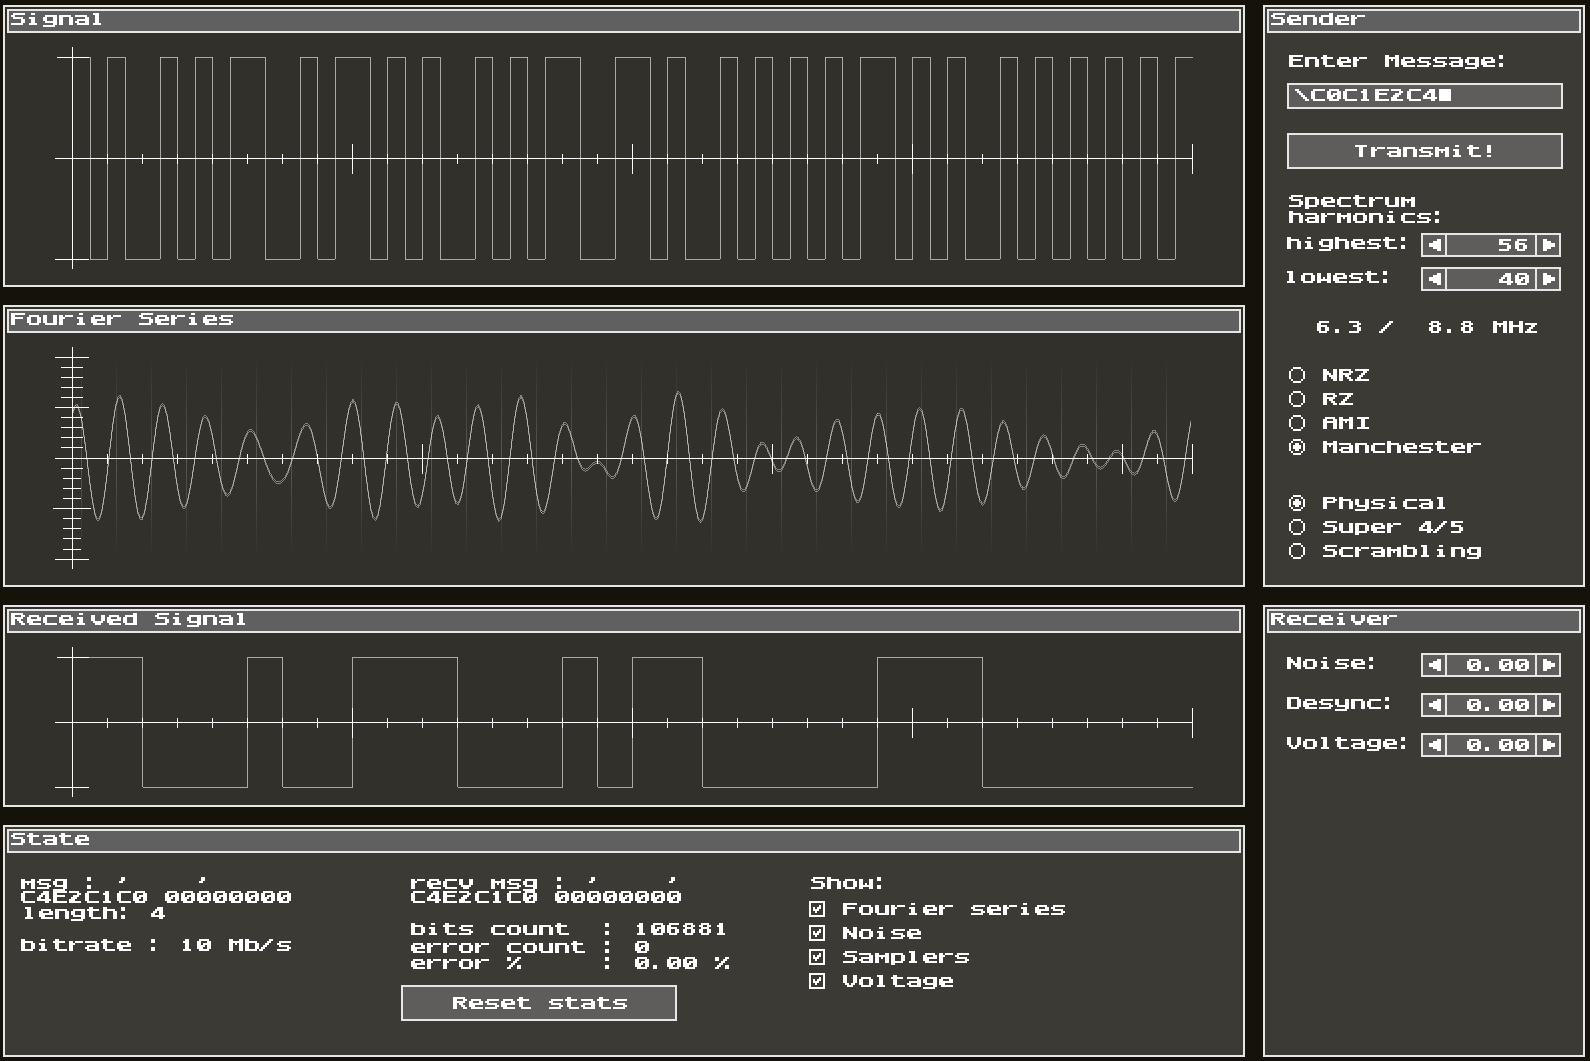
\includegraphics[width=0.95\linewidth]{./data/ideal_m2_min_f.png}
	\cutpic{0.2cm}{14cm}{./data/4_nrzS.png.jpg}
	\caption{Процент ошибок для NRZ + Scramble}
    \vspace{-4.5cm}
\end{wrapfigure}

Для NRZ+Scramble при передаче порядка 100000 бит при минимальной ширине полосы пропускания и максимально допустимых уровнях шума, рассинхронизации и граничного напряжения, процент ошибок составил 2.02\%.

\newpage
\subsection{Выводы}

На данном этапе \underline{лучшим оказался \textbf{Манчестер} (0.08\%)}, что говорит о его устойчивости к различного рода помехам.

Несмотря на то, что на предыдущем этапе NRZ был одним из лучших, в данном тесте он показал худший результат (2.36\%). Такой результат связан с тем, что на предыдущем этапе для него было получены самые высокие уровни помех, и при их совмещение метод оказался сильно подвержен ошибкам.

Такая же картина и у NRZ+Scramble – показав неплохие результаты по отдельности на прошлом этапе, при их совмещении процент ошибок оказался достаточно большим (2.02\%).

Так же объясняется и средний результат RZ и NRZ+4B/5B (1.20\% и 1.25\% соответственно). Так как они показали самые низкие уровни допустимых уровни помех, при их совмещении результат оказался лучше, чем у NRZ и NRZ+Scramble.


% -------------------------------

\section{Уровни шумов, рассинхронизации и напряжения канала связи}
В ходе этого этапа я рассчитал значения \textit{уровней шумов}, \textit{рассинхронизации} и \textit{граничного напряжения} для реального канала связи. Для этого я вычислил средние значения максимальных параметров по всем методам кодирования (округление до сотых).

\begin{enumerate}
	\item Средний уровень шума:
	      \[
		      \frac{(0.2+0.02+0.16+0.02+0.09)}{5}=0.1
	      \]

	\item Средний уровень рассинхронизации:
	      \[
		      \frac{(0.35+0.02+0.1+0.12+0.08)}{5}=0.13
	      \]

	\item Средний уровень граничного напряжения:
	      \[
		      \frac{(0.38+0.16+1+0.02+0.37)}{5}=0.39
	      \]

\end{enumerate}

Эти значения \textbf{отражают характеристики реального канала связи} с учетом использования различных методов кодирования.


% -------------------------------

\section{Полоса пропускания реального канала связи}
В ходе выполнения этого этапа я определил требуемую полосу пропускания реального канала связи. Для этого я установил рассчитанные на предыдущем этапе средние значения уровней шумов, рассинхронизации и граничного напряжения.

Затем, изменяя порядковый номер нижней гармоники от нуля и верхней гармоники от максимального значения, я определил граничные значения полосы пропускания, при которых сообщение передается без ошибок для каждого из методов кодирования. Затем определил необходимую ширину полосы пропускания для каждого метода кодирования.

\subsection{NRZ}

\begin{wrapfigure}{l}{0.63\textwidth}
	\centering
	% 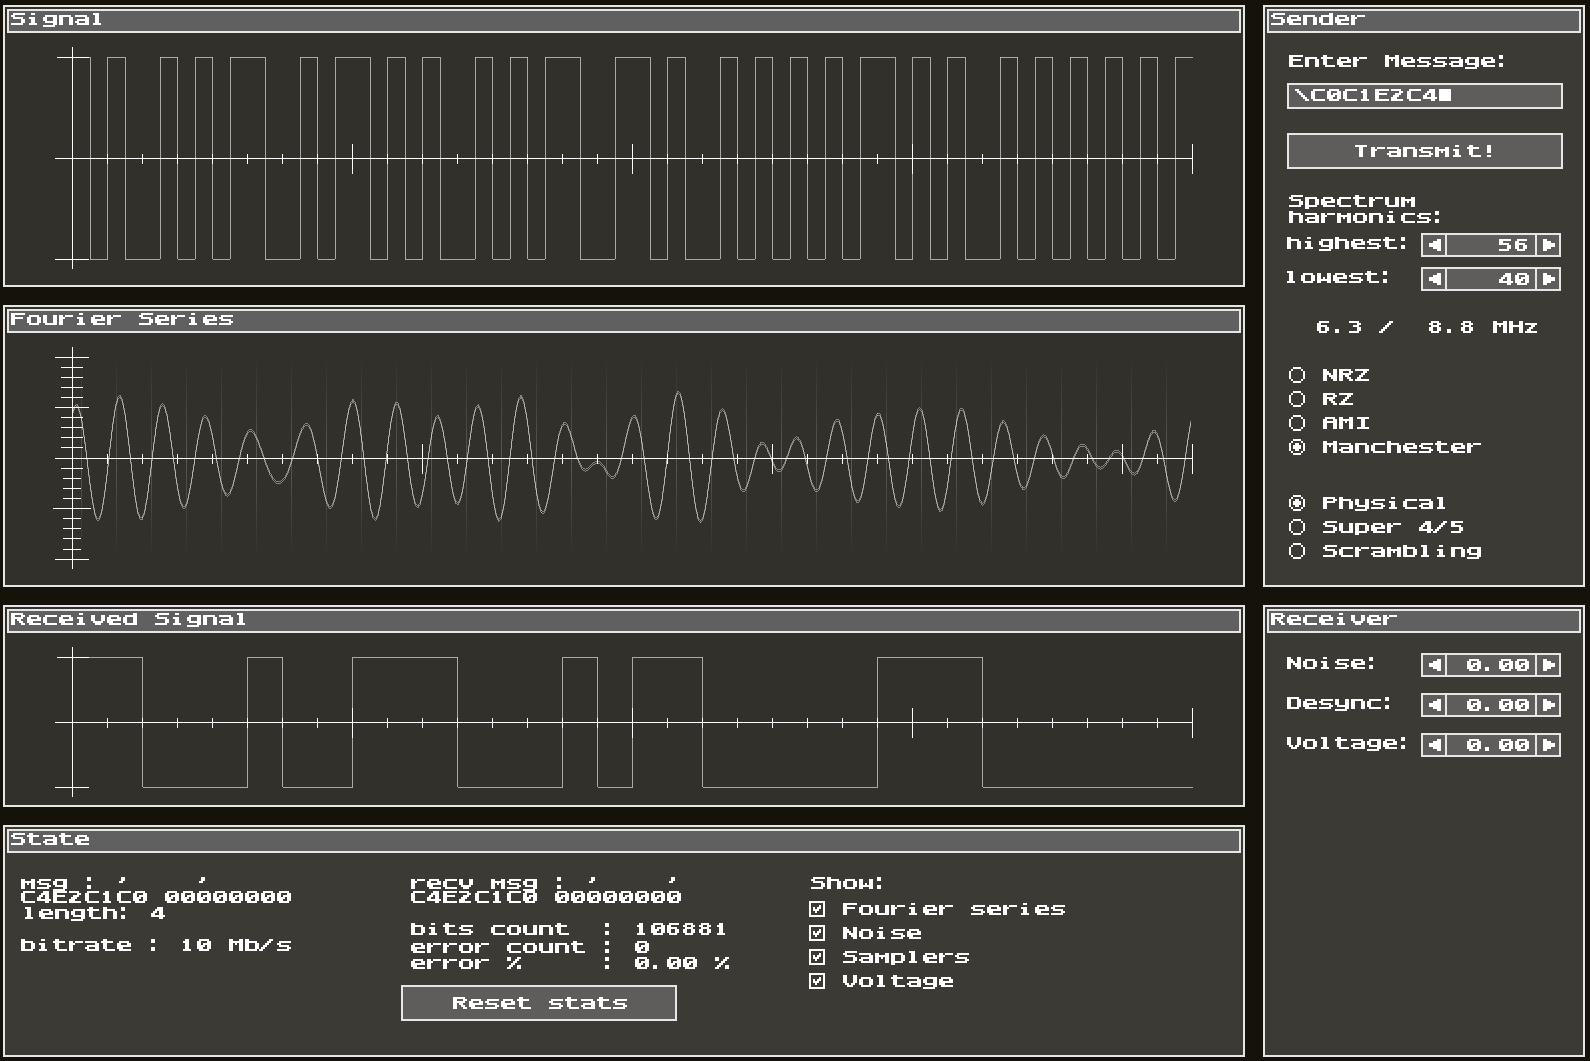
\includegraphics[width=0.95\linewidth]{./data/ideal_m2_min_f.png}
	\cutpic{0.2cm}{11cm}{./data/6_nrz.png.jpg}
	\caption{F =  1.3 - 4.4 Мгц}
    \vspace{-2.1cm}
\end{wrapfigure}

Для метода NRZ требуемая ширина полосы пропускания реального канала связи составила 3.1 МГц.
Для передачи данных без ошибок в условия реального канала связи пришлось увеличить верхнюю границу частот. Ширина полосы пропускания увеличилась с 2.5 МГц до 3.1 МГц (изменилась на +0.6 МГц).

\subsection{RZ}

\begin{wrapfigure}{r}{0.5\textwidth}
	\centering
	% 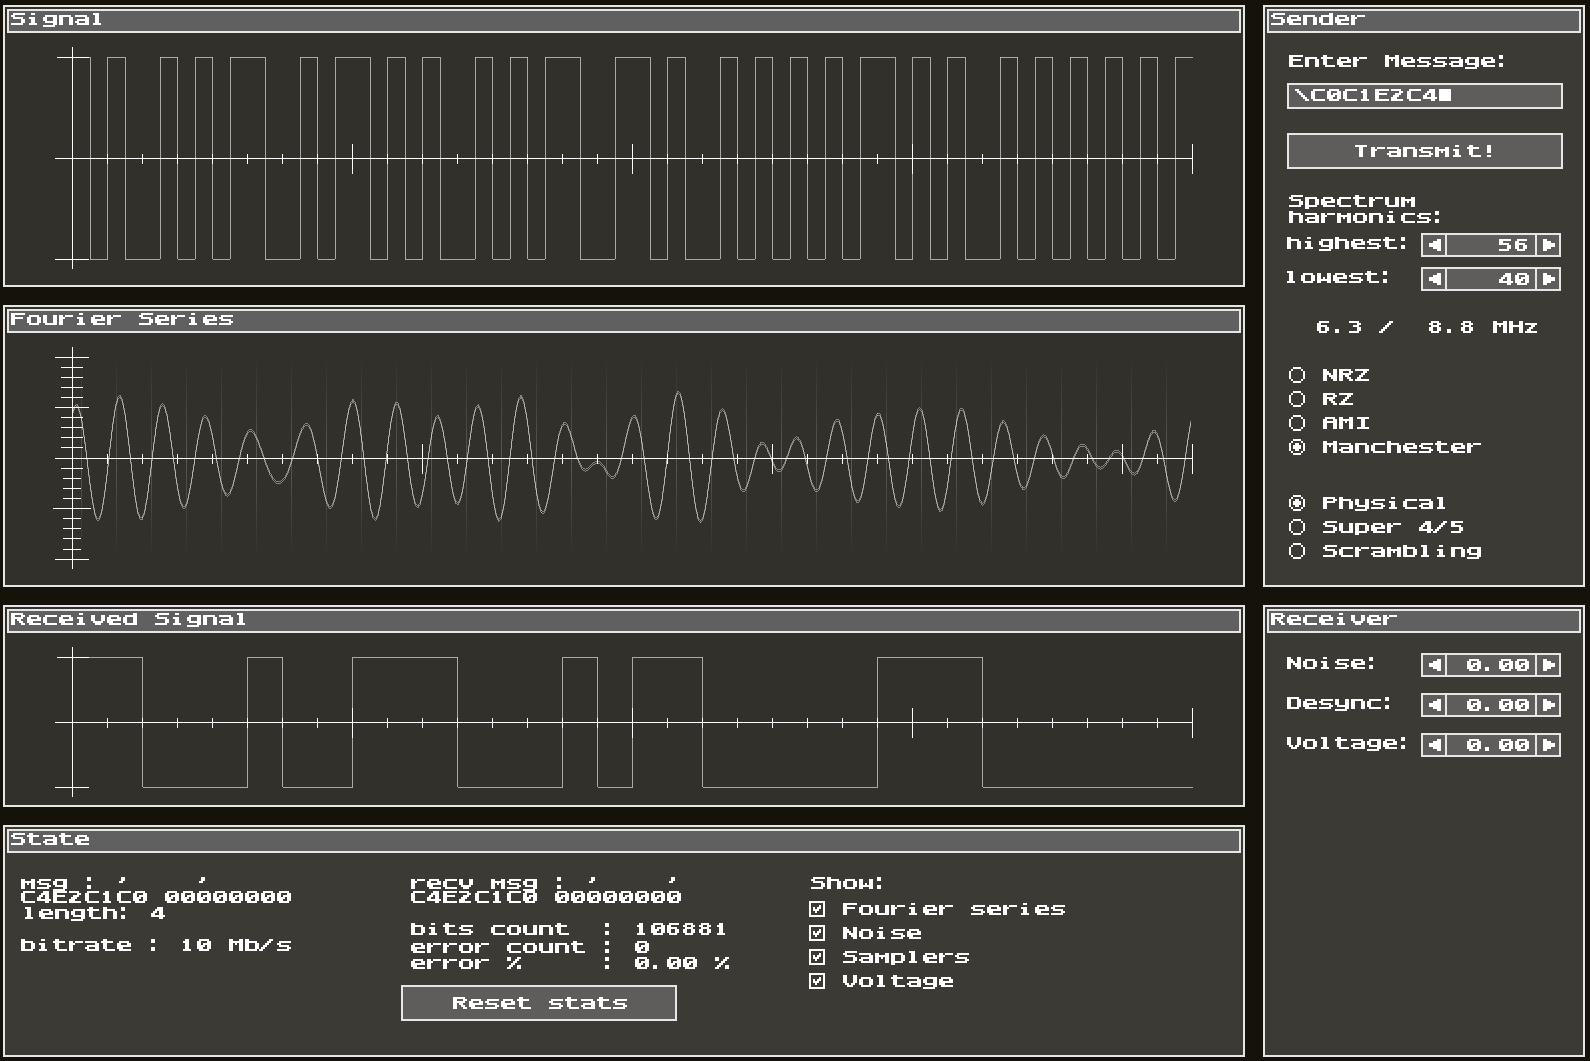
\includegraphics[width=0.95\linewidth]{./data/ideal_m2_min_f.png}
	\cutpic{0.2cm}{10cm}{./data/6_rz.png.jpg}
	\caption{F =  2.5 - 12.2 Мгц}
    \vspace{-1.7cm}
\end{wrapfigure}

\vspace{0.5cm}
Для метода RZ требуемая ширина полосы пропускания реального канала связи составила 9.7 МГц.
Для передачи данных без ошибок в реальном канале связи пришлось увеличить верхнюю границу на 3.4 МГц, а нижнюю уменьшить на 1.6 Мгц. Ширина полосы пропускания увеличилась с 4.7 МГц до 9.7 МГц (изменилась на +5 МГц). Это было необходимо для преодоления средних уровней помех, которые оказались выше, чем максимально допустимые уровни, рассчи-\\танные для данного метода на этапе 3.

\thispagestyle{empty}


\subsection{M2}

Для метода M2 требуемая ширина полосы пропускания реального канала связи составила 3.1 МГц.
Для передачи данных без ошибок в условия реального канала связи пришлось увеличить верхнюю границу на 0.6 МГц. Ширина полосы пропускания увеличилась с 2.5 МГц до 3.1 МГц (изменилась на +0.6 МГц). Это было необходимо для преодоления средних уровней помех.

\vspace{0.4cm}
\begin{figure}[H]
	\centering
	% 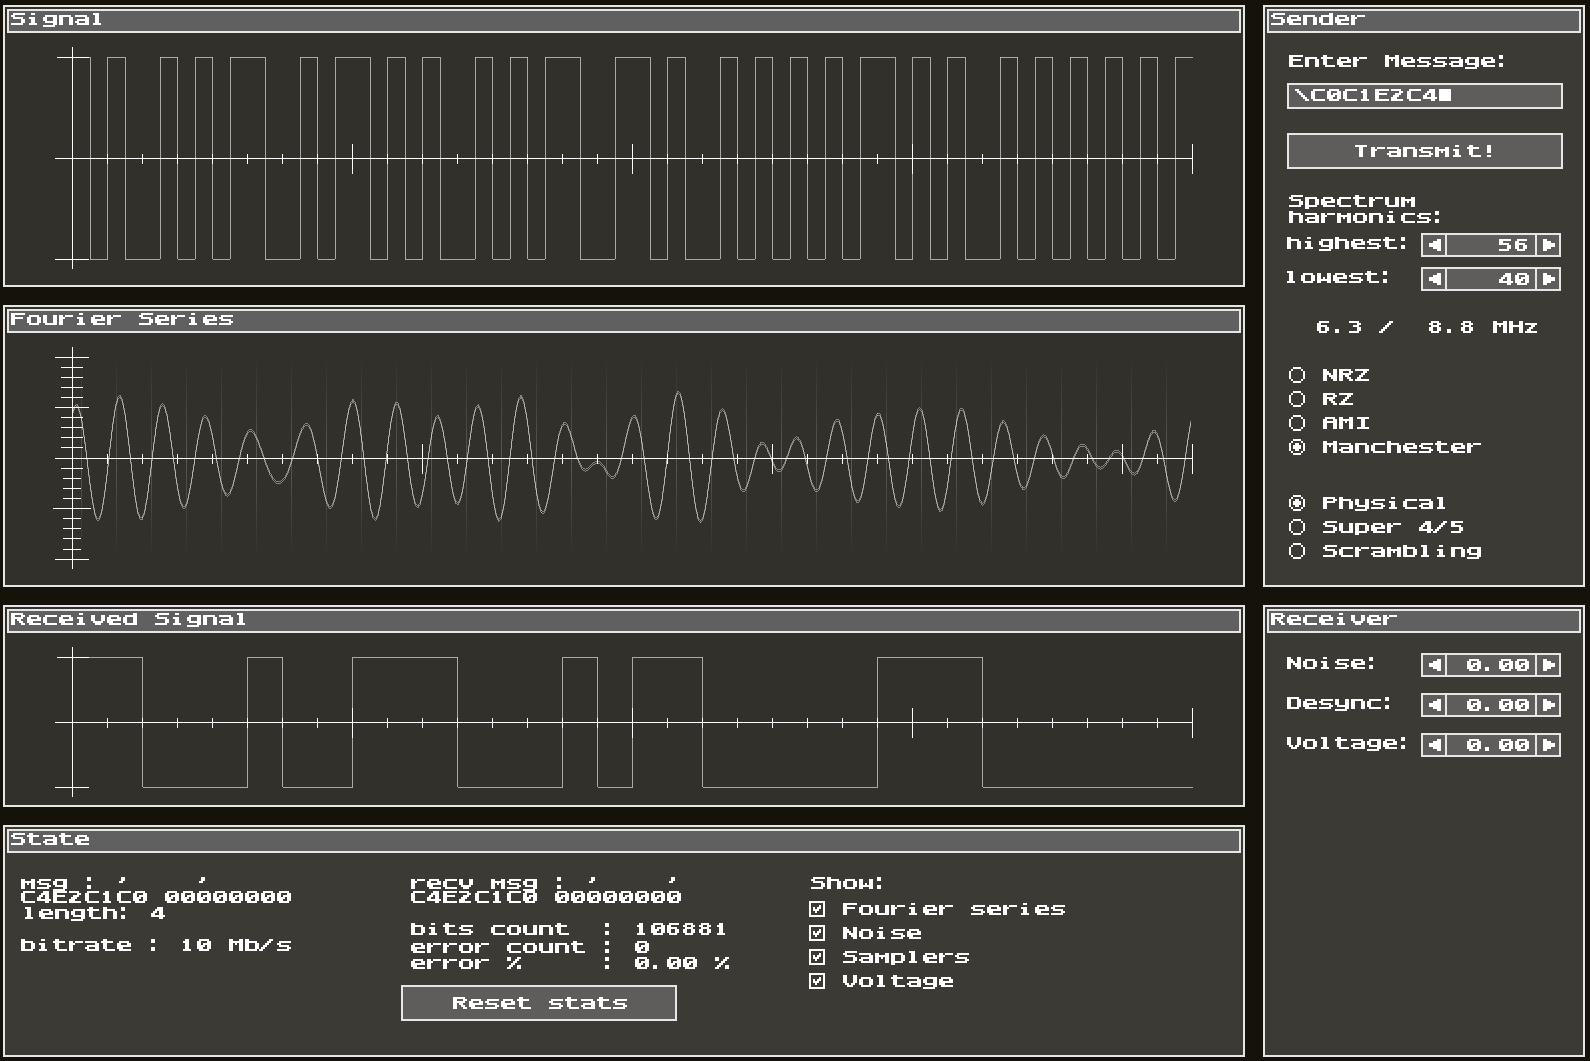
\includegraphics[width=0.95\linewidth]{./data/ideal_m2_min_f.png}
	\cutpic{0.2cm}{17.2cm}{./data/6_m2.png.jpg}
	\caption{F =  6.3 - 9.4 Мгц}
\end{figure}

\vspace{1.5cm}
\subsection{NRZ + 4B/5B}

Для метода NRZ+4B/5B требуемая ширина полосы пропускания реального канала связи составила 5.7 МГц.
Для передачи данных без ошибок в условия реального канала связи пришлось увеличить верхнюю границу на 1.5 МГц, а нижнюю уменьшить на 1.7 Мгц. Ширина полосы пропускания увеличилась с .2.5 МГц до 5.7 МГц (изменилась на +3.2 МГц). Это было необходимо для преодоления средних уровней помех, которые оказались сильно выше, чем максимально допустимые уровни, рассчитанные для данного метода на этапе 3.

\vspace{0.4cm}
\begin{figure}[H]
	\centering
	% 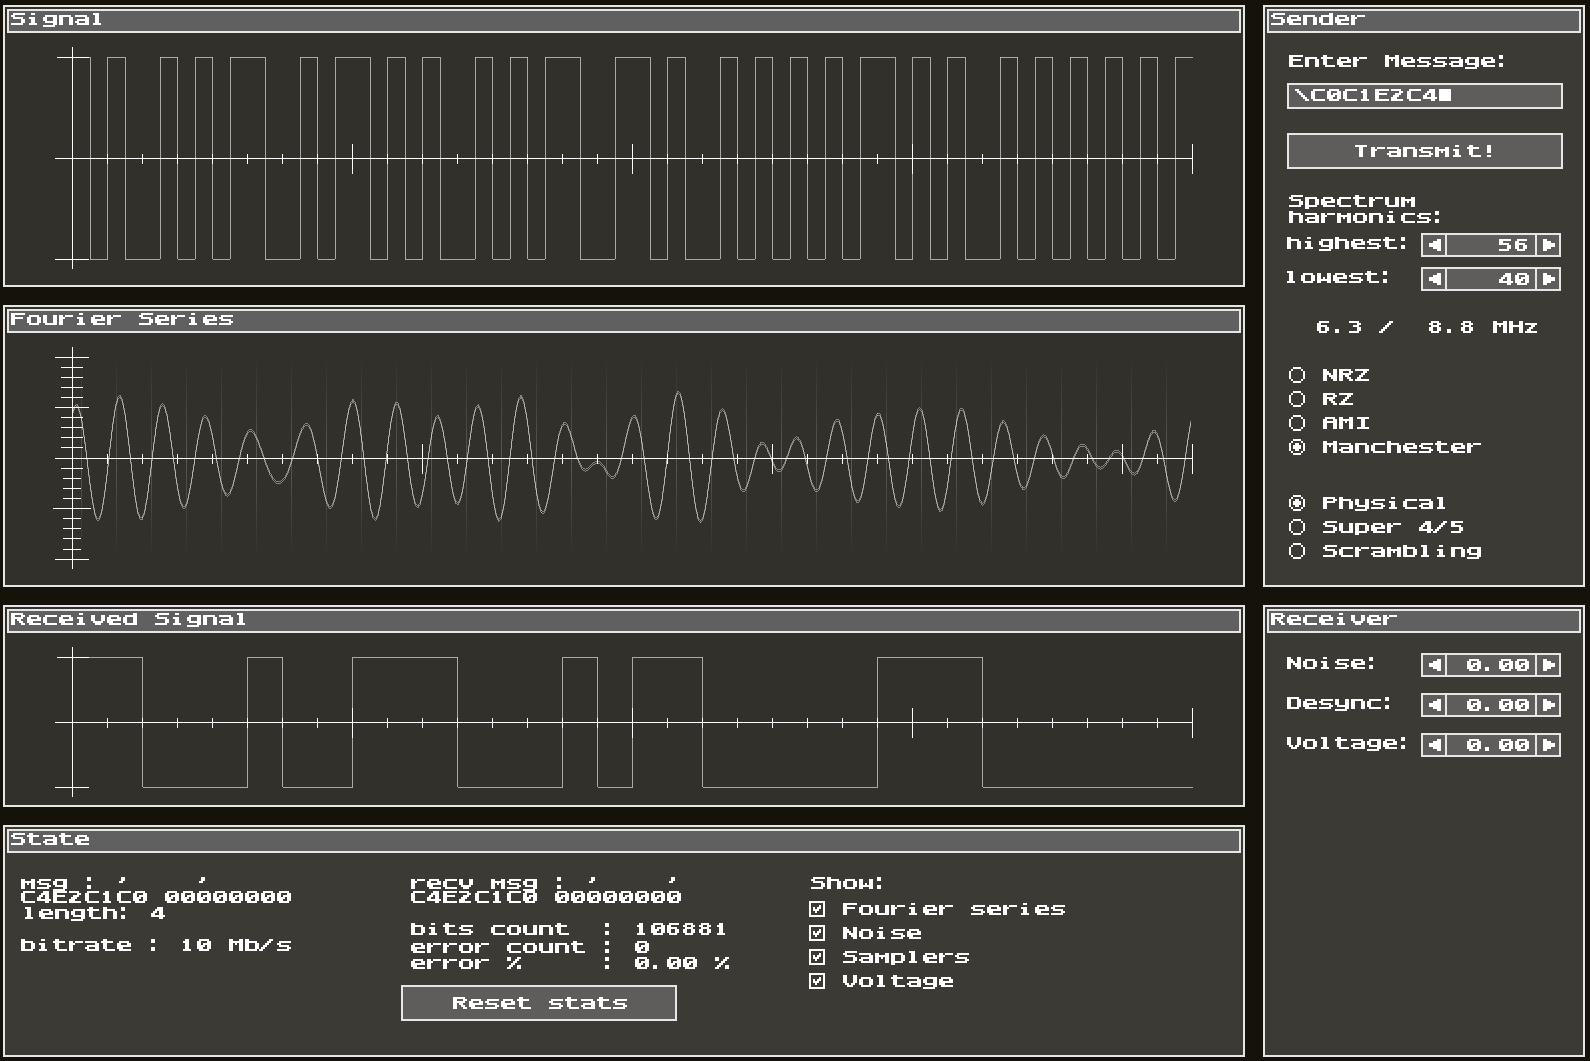
\includegraphics[width=0.95\linewidth]{./data/ideal_m2_min_f.png}
	\cutpic{0.2cm}{17.2cm}{./data/6_nrz45.png.jpg}
	\caption{F =  6.3 - 9.4 Мгц}
\end{figure}

\subsection{NRZ + Scramble}

Для метода NRZ+Scramble требуемая ширина полосы пропускания реального канала связи составила 4.4 МГц.

\vspace{0.4cm}
\begin{wrapfigure}{r}{0.6\textwidth}
	\centering
	% 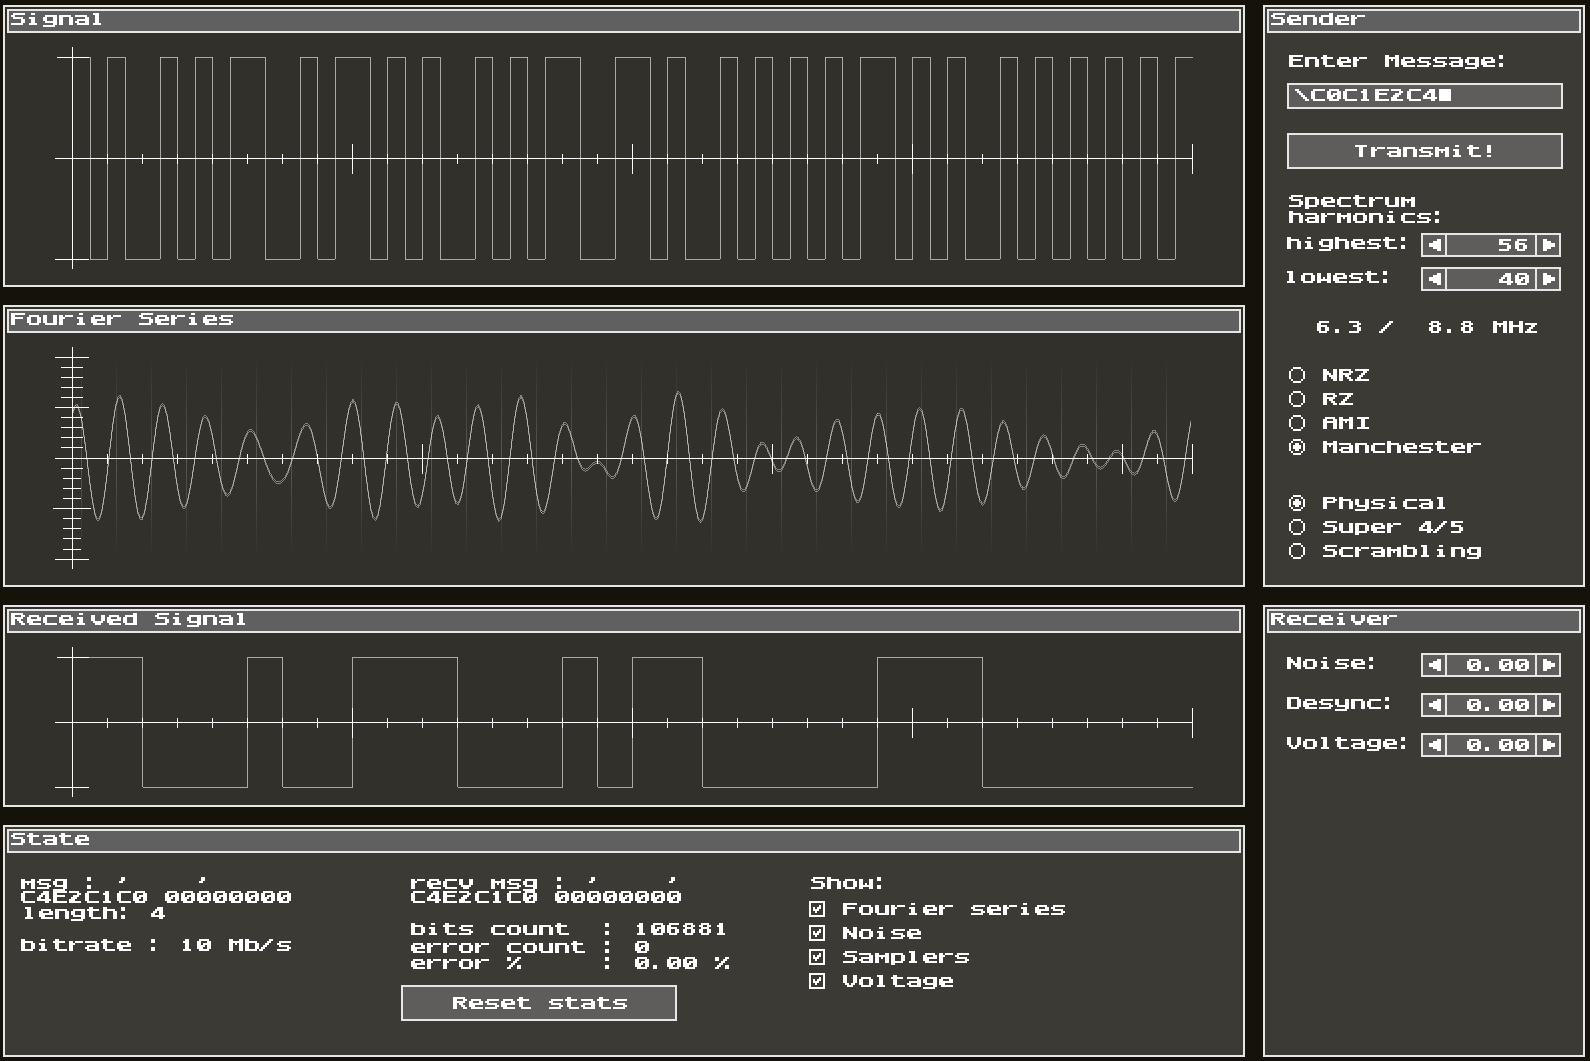
\includegraphics[width=0.95\linewidth]{./data/ideal_m2_min_f.png}
	\cutpic{0.2cm}{11.6cm}{./data/6_nrzS.png.jpg}
	\caption{F =  6.3 - 9.4 Мгц}
	\vspace{-1.7cm}
\end{wrapfigure}

Для передачи данных без ошибок в условия реального канала связи пришлось уменьшить нижнюю границу на 0.3 Мгц. Ширина полосы пропускания увеличилась с .4.1 МГц до 4.4 МГц (изменилась на +0.3 МГц). Это было необходимо для преодоления средних уровней помех, которые оказались выше, чем максимально допустимые уровни, рассчитанные для данного метода на этапе 3.

\subsection{Выводы}

Так как на третьем этапе NRZ и M2 показали наибольшие допустимые уровни помех, то при применении к ним уже средних уровней помех, их полоса пропускания не показала значительных изменений. \underline{Эти методы дали лучший} \underline{результат в \textbf{3.1 МГц}}.

На третьем этапе худшую устойчивость к помехам показали RZ и NRZ+4B/5B, поэтому при среднем уровне помех у них также худший результат по полосе пропускания – 9.7 и 5.7 МГц соответственно.

На третьем этапе NRZ+Scramble дал средний результат, поэтому при среднем уровне помех у него также средняя полоса пропускания (4.4 МГц).



% -------------------------------

\section{Сравнительный анализ}
% \begin{table}[H]
	\centering
	\scalebox{0.75}{
		\renewcommand{\arraystretch}{1.2}
		\begin{tabular}{|>{\centering\arraybackslash}m{3.8cm}|
			>{\centering\arraybackslash}m{4cm}|
			>{\centering\arraybackslash}m{3cm}|
			>{\centering\arraybackslash}m{3cm}|
			>{\centering\arraybackslash}m{3cm}|
			>{\centering\arraybackslash}m{3.5cm}|}
			\hline
			\textbf{Метод кодирования}                                                         & \textbf{Спектральные характеристики} & \textbf{Постоянная составляющая} & \textbf{Самосин- хронизация} & \textbf{Обнаруж. ошибок} & \textbf{Сложность реализации} \\
			\hline
			\textbf{Потенциальный код с инверсией при единице (NRZI)}                          &
			Малая ширина спектра ($0$--$\frac{C}{2}$), итоговый спектр $\frac{3C}{7}$          &
			Присутствует, но снижена по сравнению с NRZ                                        &
			Отсутствует, возможны проблемы при длинных последовательностях '0'                 &
			Отсутствует                                                                        &
			Низкая сложность реализации, два уровня потенциала $\implies$ низкая стоимость                                                                                                                                                                         \\
			\hline
			\textbf{Манчестерское кодирование (М2)}                                            &
			Большая ширина спектра ($0$--$C$), итоговый спектр $C$                             &
			Отсутствует                                                                        &
			Отличная, переход в середине каждого битового интервала обеспечивает синхронизацию &
			Отсутствует                                                                        &
			Средняя сложность реализации, два уровня потенциала $\implies$ умеренная стоимость                                                                                                                                                                     \\
			\hline
			\textbf{Дифф. манчестерское кодирование}                                           &
			Большая ширина спектра ($0$--$C$), итоговый спектр $C$                             &
			Отсутствует                                                                        &
			Отличная, устойчива к инверсии сигнала                                             &
			Отсутствует                                                                        &
			Высокая сложность реализации, два уровня потенциала $\implies$ умеренная стоимость                                                                                                                                                                     \\
			\hline
			\textbf{NRZI с 4B/5B кодированием}                                                 &
			Уменьшенный итоговый спектр: $\frac{C}{3}$                                         &
			Отсутствует (благодаря 4B/5B)                                                      &
			Улучшена, длинные последовательности '0' полностью устранены                       &
			Отсутствует                                                                        &
			Низкая сложность реализации, простое сопоставление битов таблицей кодировки                                                                                                                                                                            \\
			\hline
			\textbf{NRZI со скремблированием}                                                  &
			Меньше спектр, чем у изначального NRZI, но больше 4B/5B: $\frac{2C}{5}$            &
			Отсутствует (благодаря скремблированию)                                            &
			Улучшена, благодаря скремблированию, но остались длинные последовательности '0'    &
			Отсутствует                                                                        &
			Средняя сложность реализации, считать полином для каждого преобразования долго и муторно                                                                                                                                                               \\
			\hline
		\end{tabular}
	}
	\caption{Сравнение методов кодирования из этапов 2, 3 и 4}
\end{table}

\textbf{NRZI} снижает постоянную составляющую по сравнению с NRZ и сохраняет простоту реализации. Однако его эффективность сильно зависит от статистики передаваемых данных; при длинных последовательностях '0' возможны проблемы с синхронизацией, а постоянная составляющая всё ещё присутствует. Тем не менее, по сравнению с AMI, который является его прямым конкурентом, но не был рассмотрен в данном отчёте, NRZI имеет лишь два уровня потенциала, что делает его дешевле и предпочтительнее для использования.

С помощью методов логического кодирования можно существенно улучшить NRZI.

\textbf{NRZI с 4B/5B кодированием} устраняет постоянную составляющую и улучшает синхронизацию благодаря введению избыточности. Длинные последовательности нулей заменяются кодами без длительных последовательностей нулей, что повышает надёжность передачи. Спектр после 4B/5B кодирования стал $\frac{C}{3} = 3.333 \, \text{МГц}$, что на 0.7 МГц меньше, чем при скремблировании того же метода кодирования, что существенно повышает скорость передачи сообщения.

\textbf{NRZI со скремблированием} лишь частично устраняет длинные последовательности одинаковых битов, улучшая синхронизацию и также устраняя постоянную составляющую. При этом сохраняется узкая полоса пропускания, а сложность реализации существенно выше, чем у избыточного кодирования 4B/5B, а также спектр выше на 0.7 МГц.

\textbf{Манчестерское кодирование} обеспечивает отличную синхронизацию и не имеет постоянной составляющей, что повышает надёжность передачи. Однако в сравнении с NRZI с 4B/5B кодированием, мы получаем на 2/3 C меньший спектр, при этом не проигрывая в синхронизации и постоянной составляющей. Таким образом, Манчестерское кодирование получается сложнее NRZI с 4B/5B кодированием, и дороже в реализации, не имея перед ним преимуществ.

\textbf{Дифференциальное манчестерское кодирование} наследует преимущества манчестерского кодирования и дополнительно устойчиво к инверсии сигнала, что важно в шумных средах. Хотя высокая сложность реализации и широкий спектр являются его недостатками, NRZI с 4B/5B кодированием не имеет устойчивости к инверсии сигнала - оно имеет лишь частичную возможность обнаружения ошибок за счёт наличия запрещённых символов. Исходя из этого, если важно иметь устойчивость к инверсии сигнала и есть возможность пожертвовать спектром, а соответственно более низкой скорости передачи сообщения, то предпочтительнее будет выбрать Дифференциальное манчестерское кодирование.




% -------------------------------

\section{Выводы}
% В результате применения логического кодирования и скремблирования к исходному сообщению при использовании метода NRZI удалось значительно улучшить характеристики сигнала по сравнению с исходным методом NRZI. Благодаря избыточному кодированию 4B/5B и скремблированию были устранены длинные последовательности нулей, что повысило надёжность синхронизации и устранило постоянную составляющую сигнала. При этом сохраняется узкая полоса пропускания и низкая сложность реализации, что делает эти методы эффективными для использования в системах с ограниченными ресурсами и требованиями к полосе пропускания.

По сравнению с манчестерскими методами кодирования, NRZI с логическим кодированием или скремблированием обеспечивает более эффективное использование полосы пропускания, так как требует меньшей ширины спектра. Однако манчестерское и дифференциальное манчестерское кодирование всё ещё превосходят по надёжности синхронизации и устойчивости к помехам, что делает их предпочтительными в системах, где эти факторы являются критически важными.

Таким образом, применение логических кодирований и скремблирования позволяет улучшить характеристики методов с низкой сложностью реализации, не имеющих надёжной синхронизации и обнаружения ошибок, приближая их по качеству к более сложным методам, таким как манчестерское кодирование. Выбор между этими методами должен основываться на конкретных требованиях системы передачи данных, включая допустимую полосу пропускания, сложность реализации и необходимость в надёжной синхронизации.


\end{document}
